\documentclass{beamer}
\usepackage{caption}
\usepackage{graphicx}
\usepackage{comment}
%\usepackage{fontspec}

%\setmainfont{} % Replace "Arial" with your desired font

% \usepackage{beamerthemesplit} // Activate for custom appearance

\usetheme{Singapore}
%\usefonttheme{professionalfonts}

\title{Potensialer og addert masse \\Krefter og Respons i hiv}
\author{Ole}
\date{Vår 2025}

\begin{document}

\frame{\titlepage}

\section[Outline]{} %I denne oppgaven ser vi på en flytende geometri i to dimensjoner. Vi regner først på kreftene fra en geometri i bevegelse til stillestående vann. Så regner vi på kreftene som mottas og reflekteres av en stillestående geometri. Vi undersøker resonans og repons i hiv.
\frame{\tableofcontents}

\section{Del 1 - Geometri som beveger seg i fluid}
\subsection{Randverdi i 2D}
\begin{frame}
  \frametitle{Randverdi i 2D}
  Vi har en geometri som beveger seg med en fart U i et ubegrenset fluid. Bevegelsen i fjernfeltet er null. 
Løsningen på problemet finnes ved å løse integrallikningen:
\begin{equation}
    -\pi \phi(\bar{x},\bar{y})  + \int_{S_B} \phi  \frac{\partial }{\partial n} \ln r dS = \int_{S_B}  \frac{\partial \phi}{\partial n} \ln r dS
\end{equation} %mikkel sier $phi_i$... 
der $\partial \phi / \partial n = n_1$ langs med $S_B$. %$r = x - \bar{x} , y -\bar{y}$
\end{frame}

\begin{frame}
  \frametitle{Likninger på diskret form}
 Potensialet
\begin{equation}
    -\pi \phi_n  + \Sigma_{m=1}^N \phi_m (-\Delta \Theta_{n,m})   =  \sum_{m=1}^N [\frac{\partial \phi}{\partial n}]_m h_{n,m}
\end{equation}

Addert masse kan approksimeres slik:
\begin{equation}
    m_{ij}  = -\rho \int_{S} \phi_j n_i dS \, \simeq \, -\rho \sum_{m=1}^N [\phi_j]_m  [n_i]_m \Delta S_m.
\end{equation}

\end{frame}
% - % - % - % - % - %
\subsection{Sirkel}
\begin{frame}
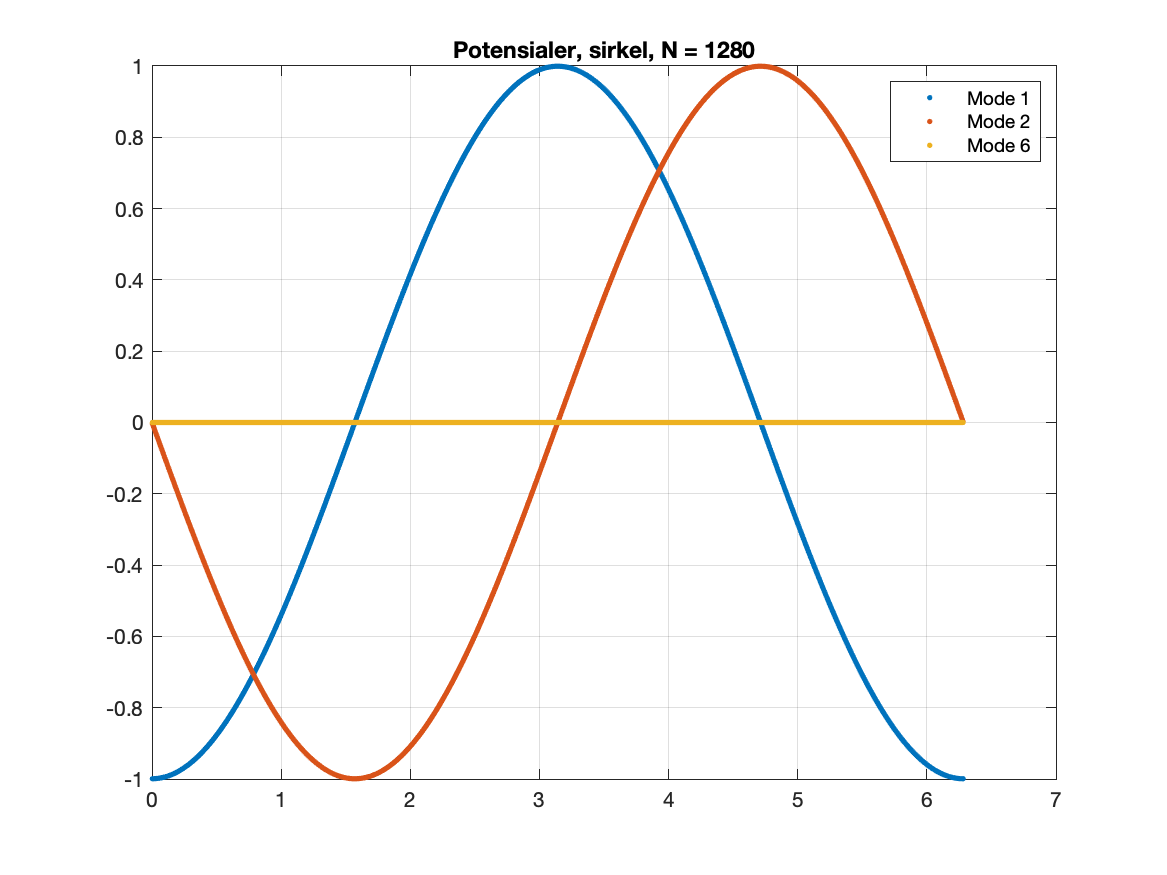
\includegraphics[width=0.8\linewidth]{/Users/ole/Tex/MEK4420/oblig1images/potensialer_sirkel.png}
\end{frame}

\begin{frame}
{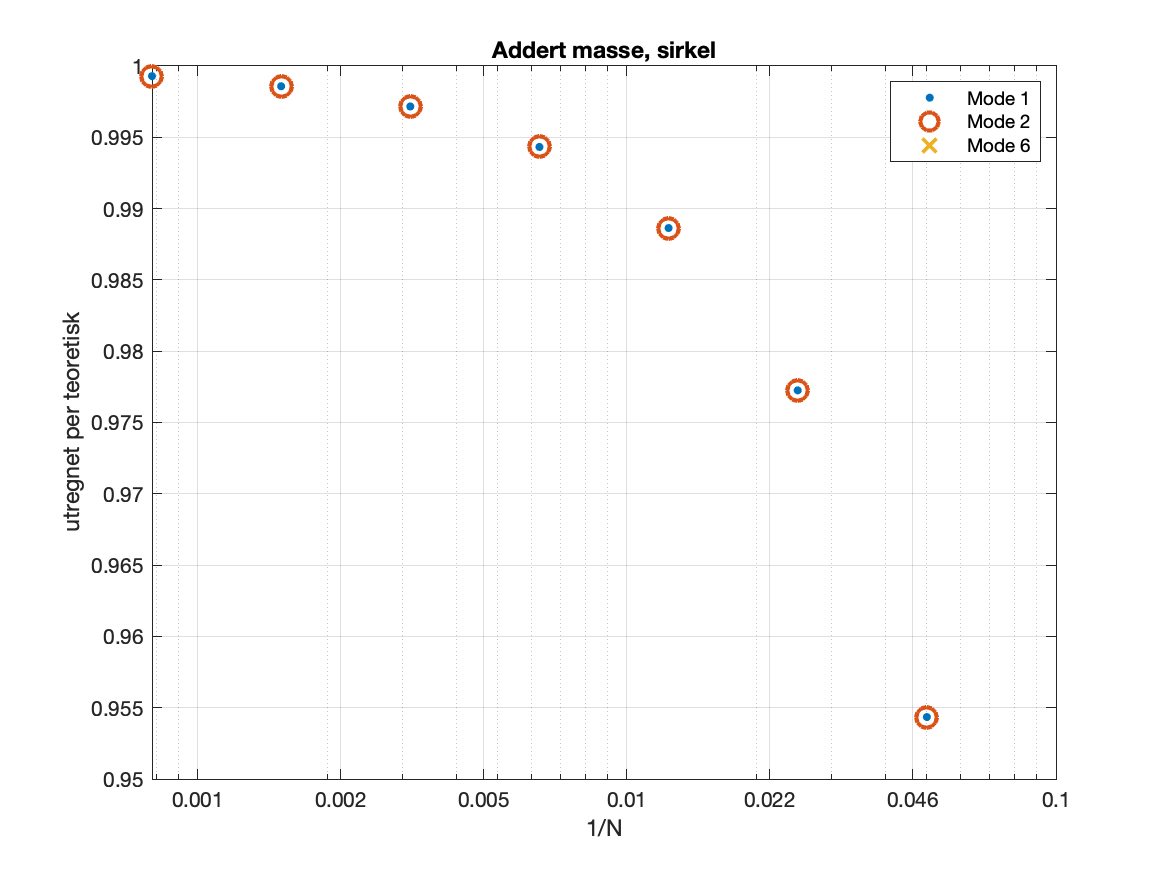
\includegraphics[width=0.8\linewidth]{/Users/ole/Tex/MEK4420/oblig1images/m11_sirkel.png}}
Allerede ved første diskretisering, N=20, så har vi over 95\% samsvar mellom teoretisk og utregnet. 
\end{frame}

% - - - Ellipse - - - %
\subsection{Ellipser}
\begin{frame}
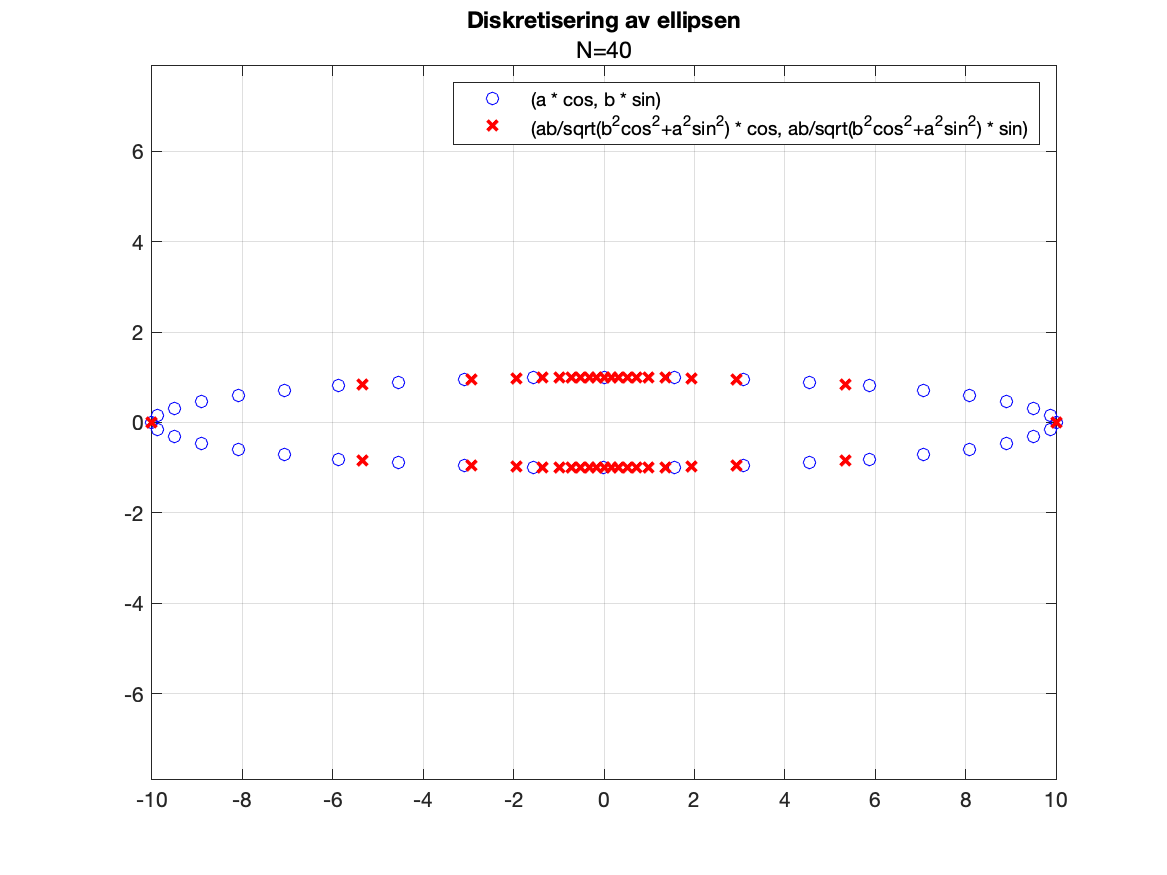
\includegraphics[width=0.8\linewidth]{/Users/ole/Tex/MEK4420/oblig1images/diskretisering_ellipse.png}
\end{frame}

\begin{frame}
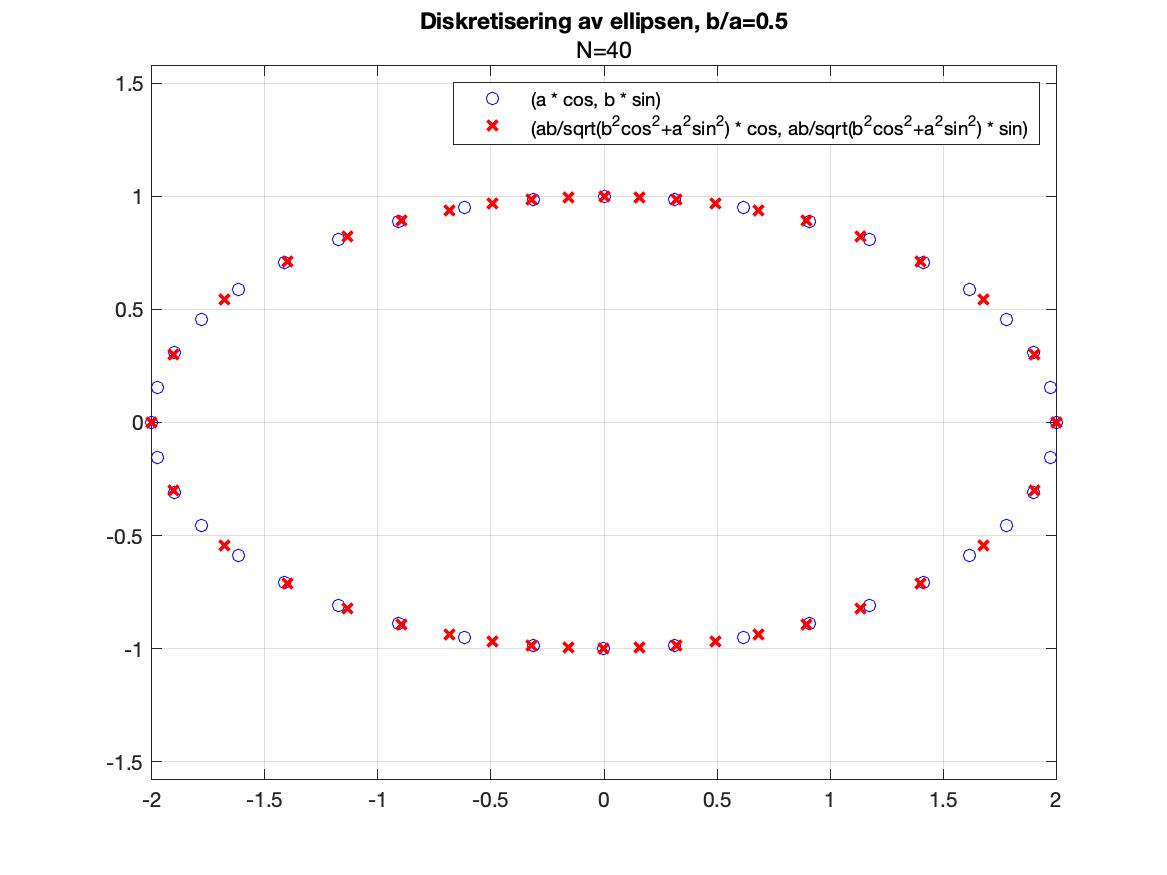
\includegraphics[width=0.8\linewidth]{/Users/ole/Tex/MEK4420/oblig1images/diskretisering_2ellipse.png}
\end{frame}

\begin{frame}
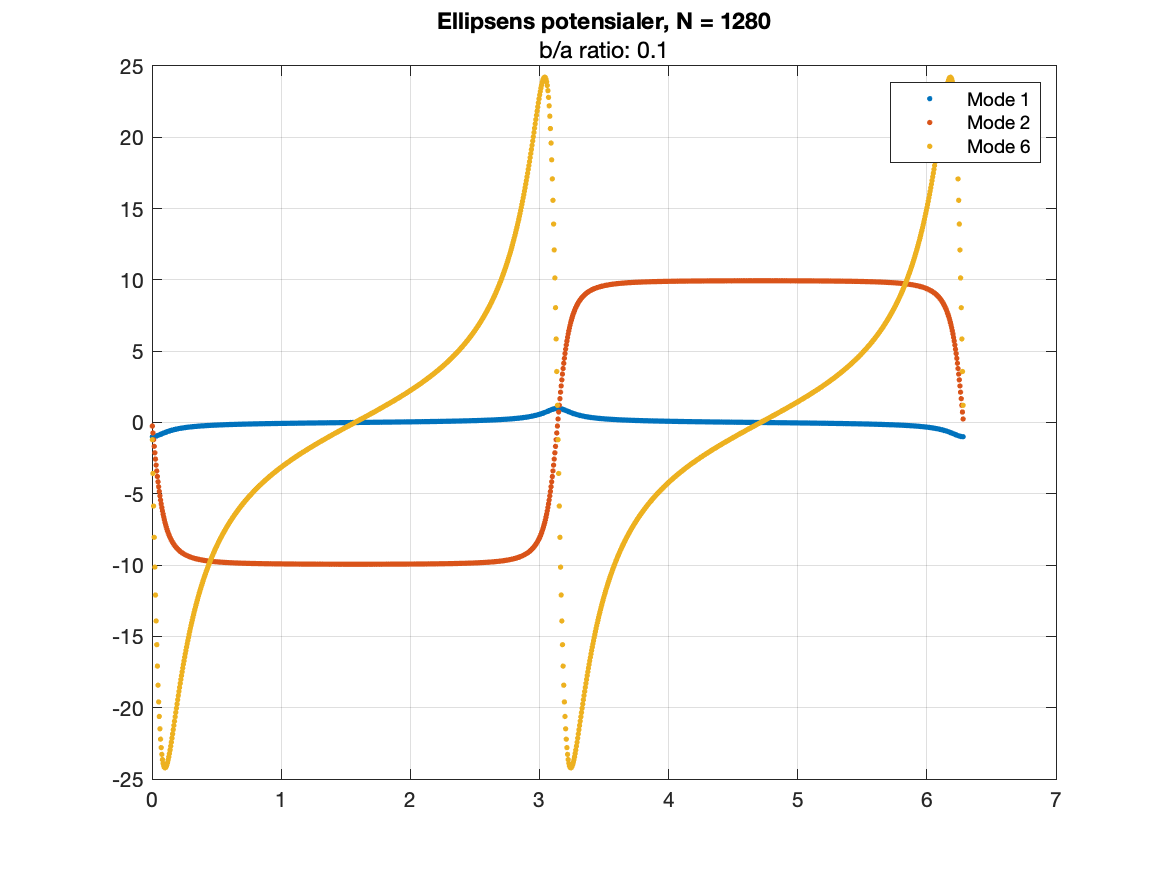
\includegraphics[width=0.8\linewidth]{/Users/ole/Tex/MEK4420/oblig1images/potensialer_ellipse.png}
\end{frame}

\begin{frame}
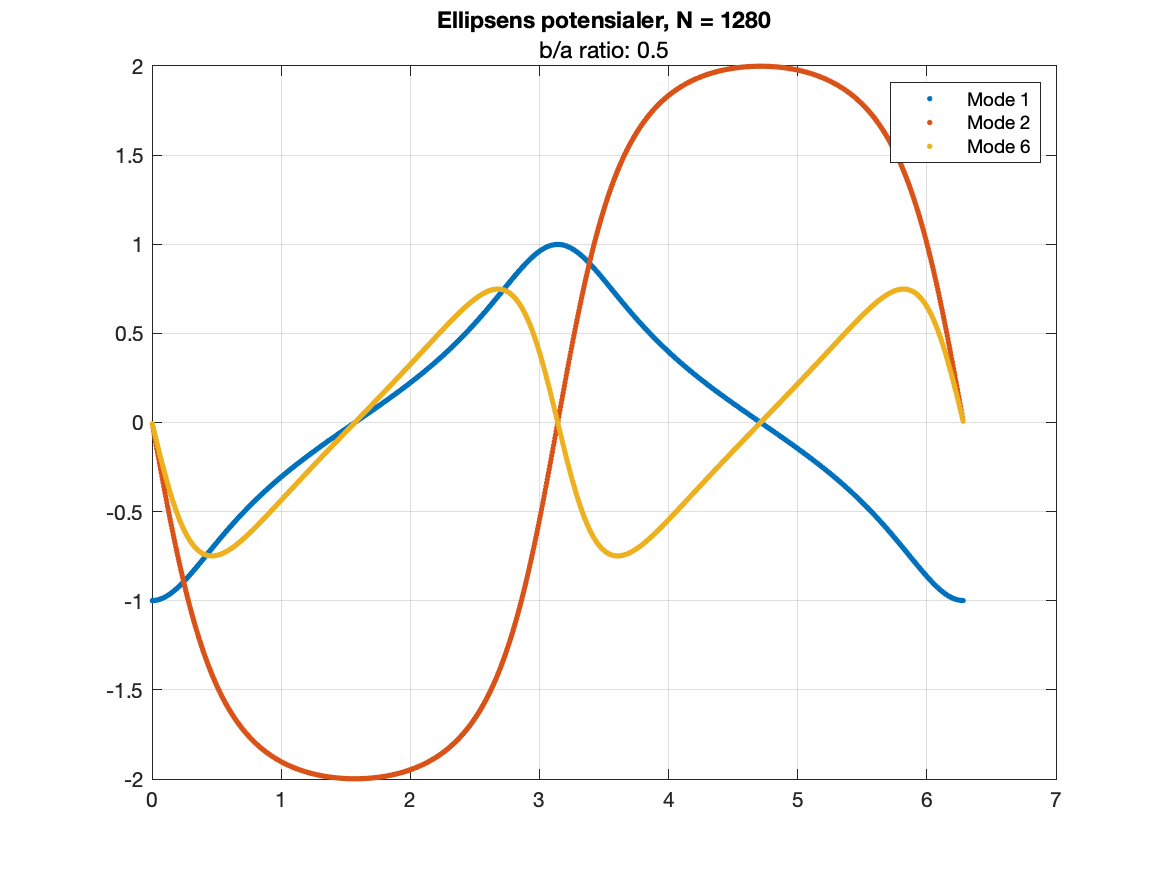
\includegraphics[width=0.8\linewidth]{/Users/ole/Tex/MEK4420/oblig1images/potensialer_2ellipse.png}
\end{frame}

\begin{frame}
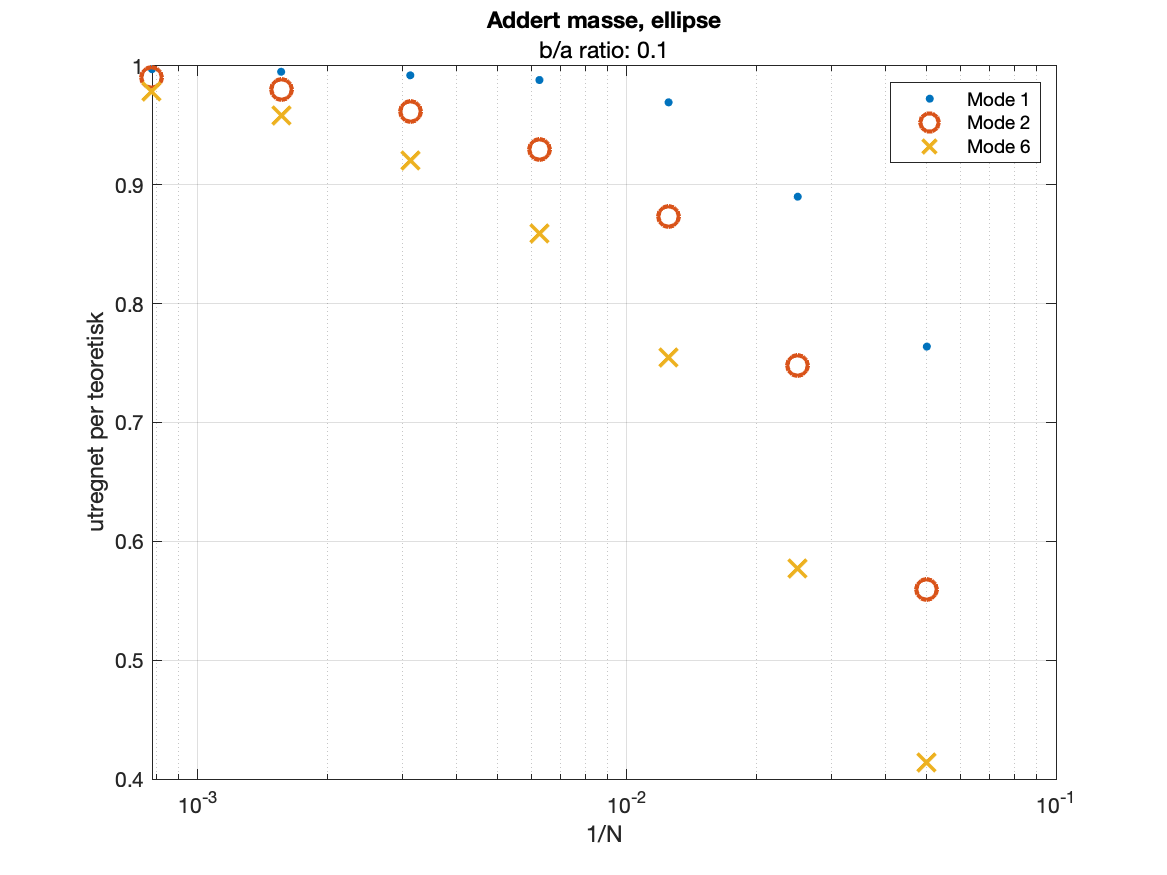
\includegraphics[width=0.8\linewidth]{/Users/ole/Tex/MEK4420/oblig1images/m11_ellipse.png}

N = 20,40,80,160,320,640,1280. 
\end{frame}

\begin{frame}
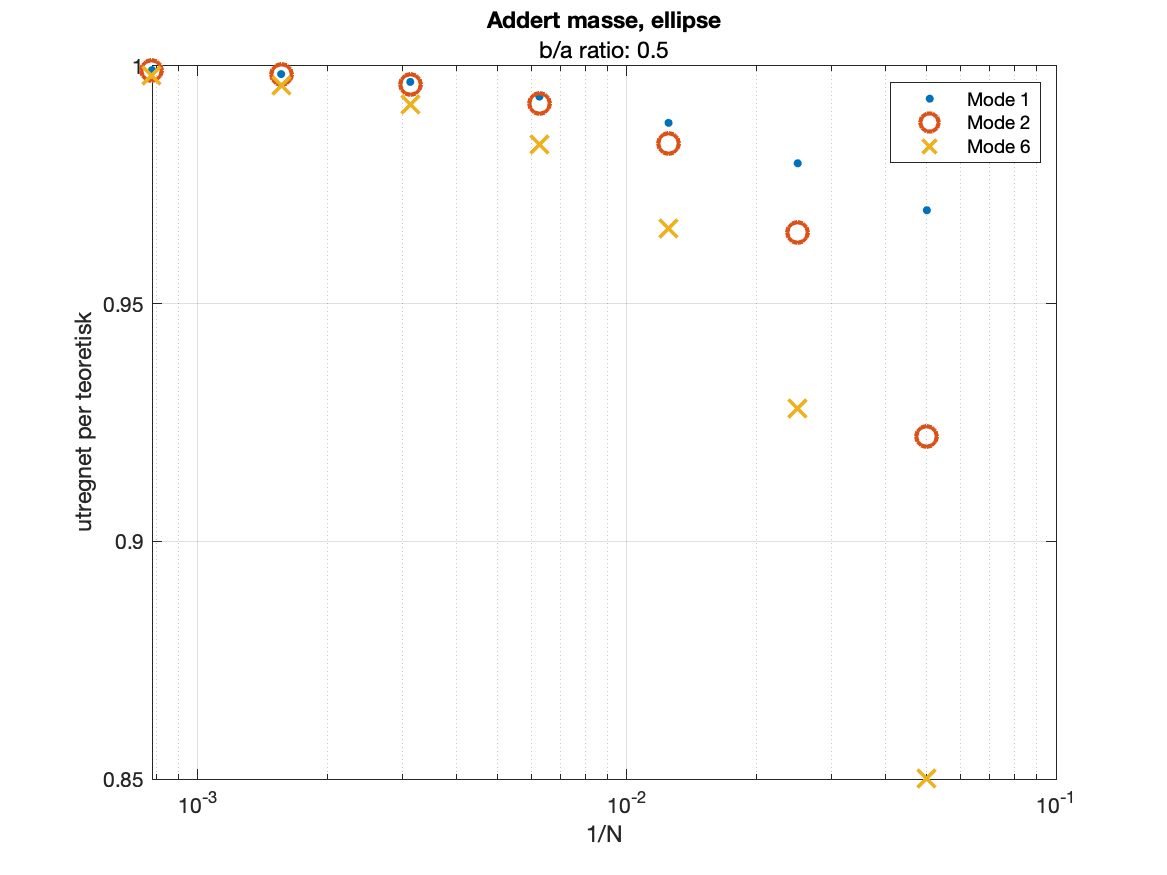
\includegraphics[width=0.8\linewidth]{/Users/ole/Tex/MEK4420/oblig1images/m11_2ellipse.png}

N = 20,40,80,160,320,640,1280.
\end{frame}




% - - - KVADRAT - - - %
\subsection{Kvadrat}
\begin{frame}
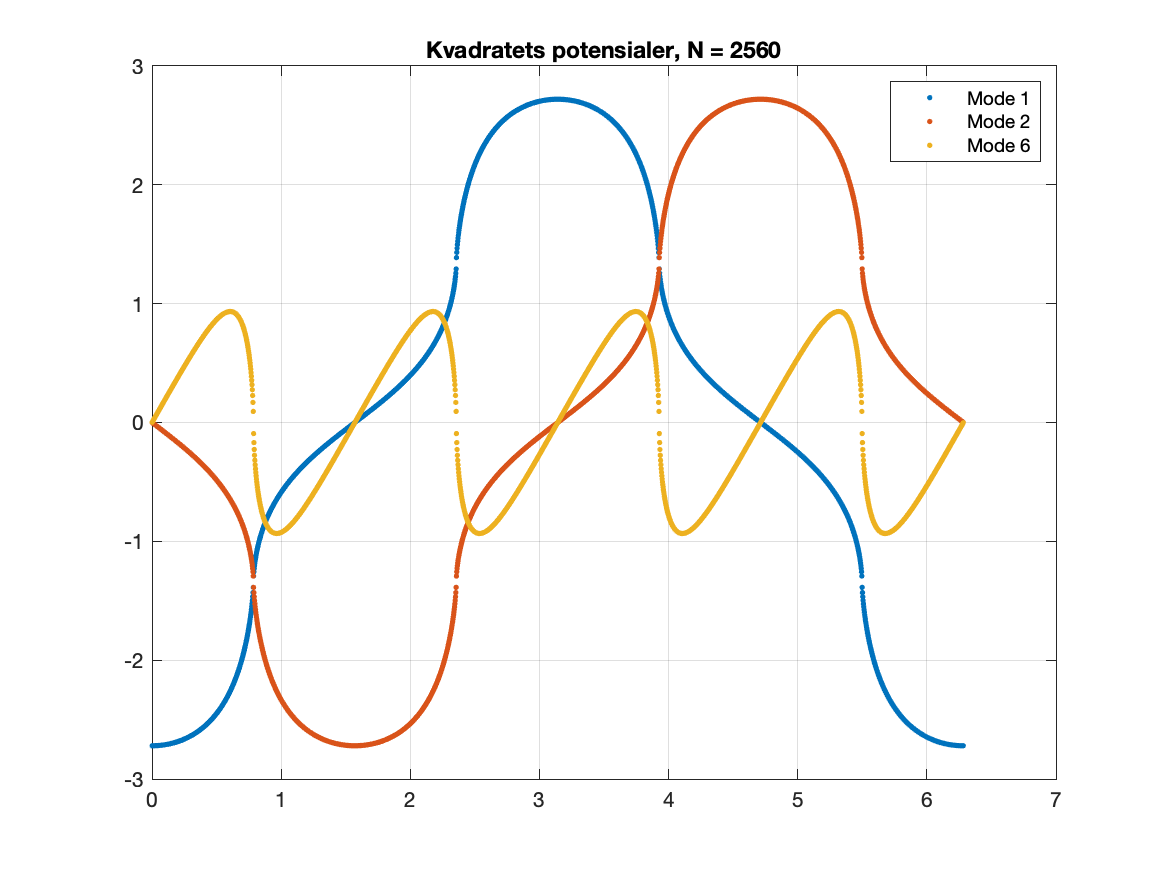
\includegraphics[width=0.8\linewidth]{/Users/ole/Tex/MEK4420/oblig1images/potensialer_kvadrat.png}
%Kvadratets potensialer i horisontal og vertikal retning er like. Rotasjonen viser tydelig samme utslag ved hvert hjørne
\end{frame}
\begin{frame}
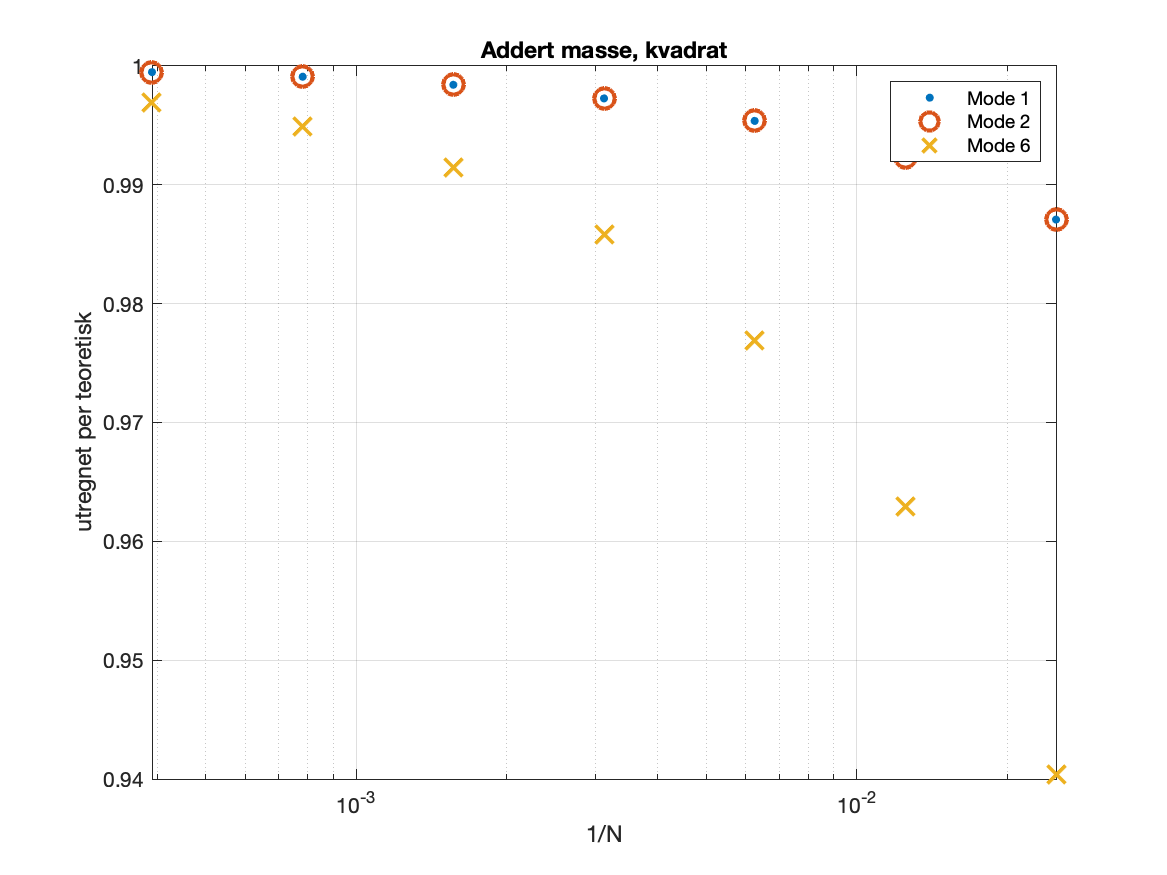
\includegraphics[width=0.8\linewidth]{/Users/ole/Tex/MEK4420/oblig1images/m11_kvadrat.png}
%På kvadratet har det blitt brukt ett hakk flere N. Verdier for
 
N = 40,80,160,320,640,1280,2560.
\end{frame}


\begin{frame}
Vi har sett på 3 geometrier: sirkel, ellipse, og kvadrat. Vi har sett at den utregnede adderte massen konvergerer mot den teoretiske, med ulik hastighet, når vi øker N diskretiseringspunkter. Det er fasongen på geometrien som avgjør den adderte massen. 
\end{frame}




%%%%%%%%%%%%%%%%%%%%%%%%%%%%
%%%%%%%%%%% ... DEL 2 ... %%%%%%%%%%%
%%%%%%%%%%%%%%%%%%%%%%%%%%%%
\section{Del 2 - Krefter og respons i hiv}
\begin{frame}
  \frametitle{Del 2 - Krefter og respons i hiv}
  Vi ønsker å se på kreftene som virker på et flytende legme. Kun i hiv. 
  \begin{enumerate}
  \item Radiasjonsproblemet
  \item Diffraksjonsproblemet
  \item Respons i hiv
  \end{enumerate}
\end{frame}

\subsection{Radiasjonsproblemet}
\begin{frame}
  \frametitle{Radiasjonsproblemet}
  Radiasjonspotensialet er gitt ved 
  \begin{equation}
	\Phi_R(x,y,t) = Re\Big( \mathrm{i} \omega \xi_2 \phi_2(x,y) e^{\mathrm{i} \omega t} \Big), 
  \end{equation}
  Randbetingelsene for problemet.  %nevne at det kommer fra Bernoulli?
  \begin{enumerate}
  \item Kinematisk grensebetingelse: $g \frac{\partial \phi_2}{\partial y} = - \omega^2 \phi_2$
  \item Uendelig dyp: $|\nabla \phi_2| \to 0$, når $y \to - \infty$
  \item Fluidet er inkompressibelt, uten virvling. LAPLACE $\nabla^2 \phi_2  = 0$ i fluidet.      
  \end{enumerate}
 %Randverdiene for Green-funksjonen, men i 
 Vi konstruerer en GREEN-funksjon som oppfyller de samme randbetingelsene, bortsett fra i en liten omegn om singulariteten. 
\end{frame}

\begin{frame}{Bølge-Green-funksjon}
\begin{align*}
	g(x,y; \bar{x}, \bar{y}, t) = Re\big( G(x,y; \bar{x}, \bar{y}, t) e^{\mathrm{i} \omega t} \big),\\
	G(x,y; \bar{x}, \bar{y}, t) =\log (r/r_1) + Re(f_1) + i Re(f_2), \\ 
	r = \sqrt{(x- \bar{x})^2 + (y- \bar{y})^2}
\end{align*}
%Bruker $z = x + \mathrm{i}  y$ og $\bar{\zeta }^* = \bar{x} -\mathrm{i}  y$

\begin{align*}
f_1 &= 2PV \int_0^{\infty} \frac{e^-\mathrm{i} k(z-\bar{\zeta }^*) }{K-k} dk = -2e^Z(E_1(Z) + \log Z - \log(-Z)) \\
f_1 &\rightarrow \pm 2 \pi e^Z, x-\bar{x} \rightarrow\pm\infty \\
f_2 &= 2 \pi e^Z \\
Z &= K(y +\bar{y}) - \mathrm{i} K (x- \bar{x})
\end{align*}
 
\end{frame}


% - % - % - % - % - % Diskretisering
\begin{frame}
    \begin{minipage}[t]{0.45\linewidth}
        \centering
        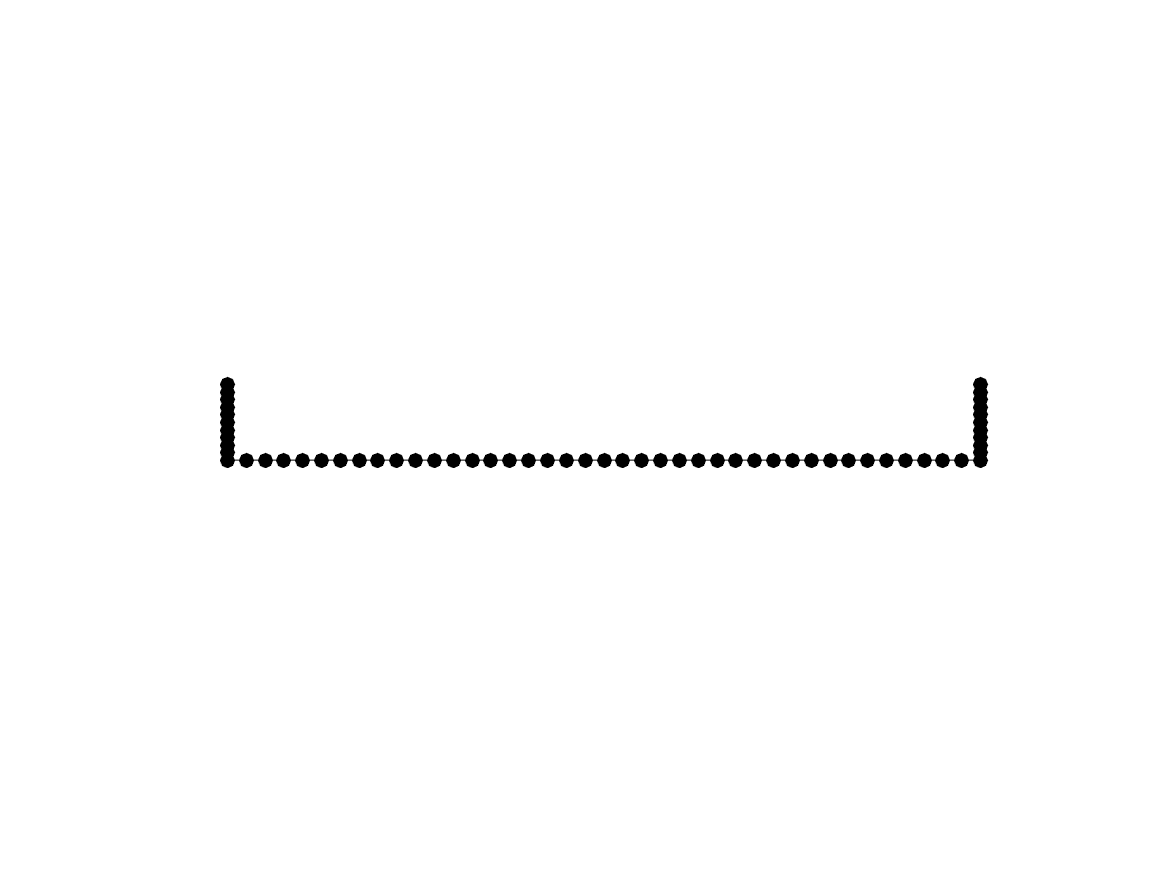
\includegraphics[width=\linewidth]{/Users/ole/Tex/MEK4420/oblig2images/boxes_1.png}
        \captionof{figure}{L/D = 10}
    \end{minipage}
    \hspace{0.05\linewidth} 
    \begin{minipage}[t]{0.45\linewidth}
        \centering
        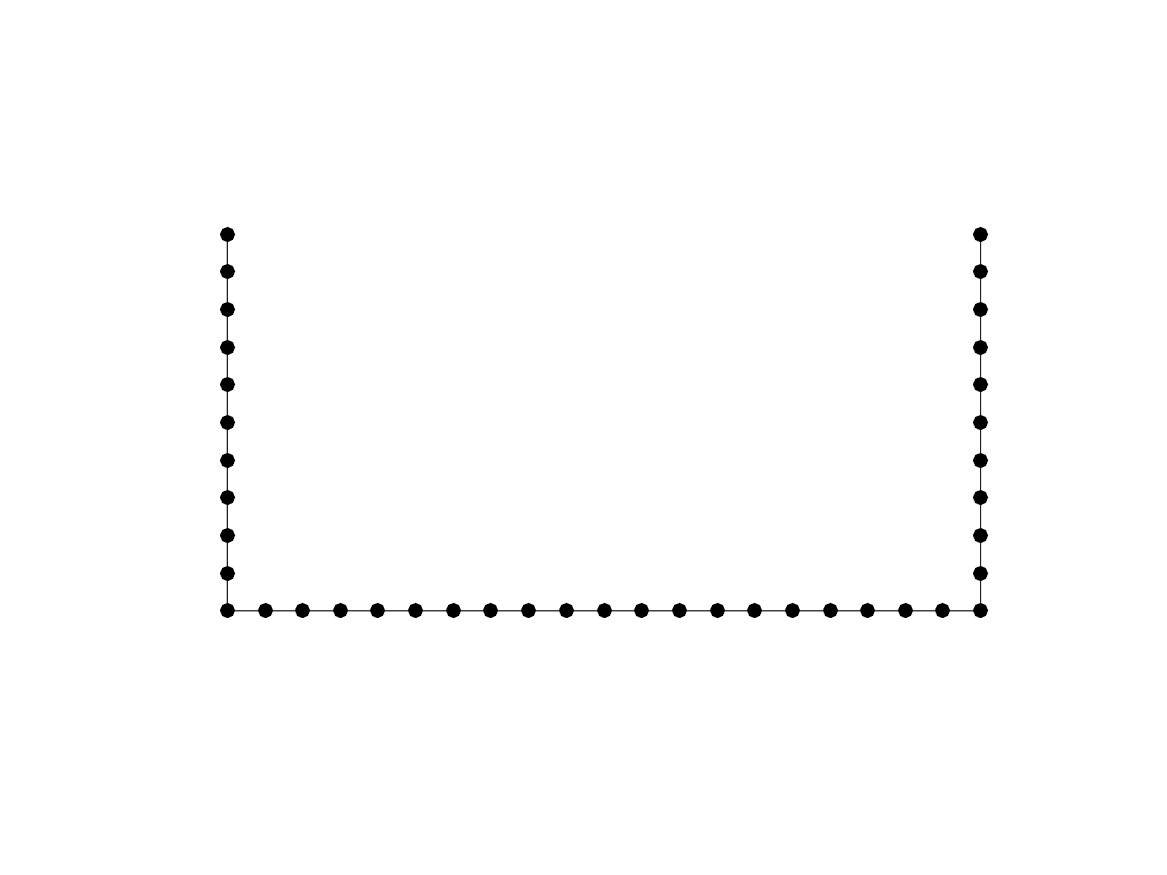
\includegraphics[width=\linewidth]{/Users/ole/Tex/MEK4420/oblig2images/boxes_2.png}
        \captionof{figure}{L/D = 2}
    \end{minipage}
    \vspace{-0.2cm}  % Adjust vertical space for overlap
    \begin{minipage}[t]{0.45\linewidth}
        \centering
        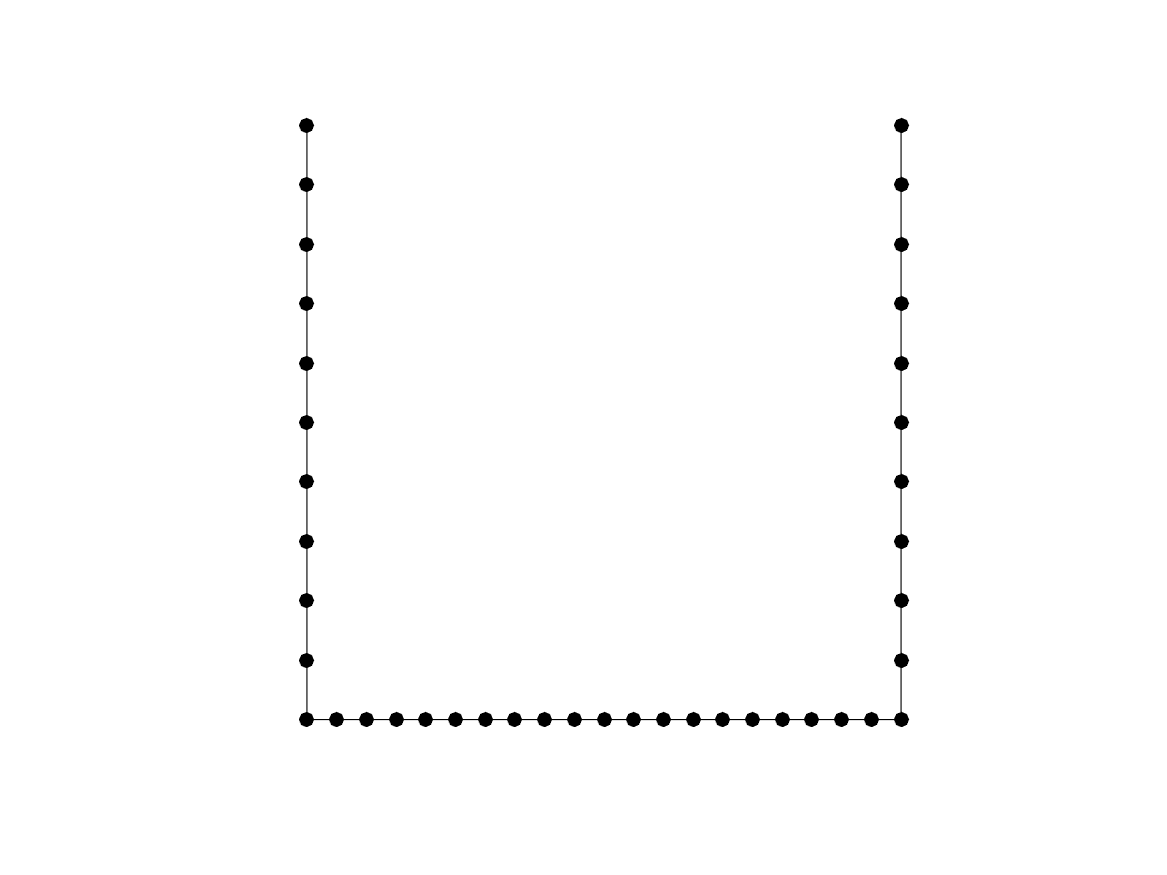
\includegraphics[width=\linewidth]{/Users/ole/Tex/MEK4420/oblig2images/boxes_3.png}
        \captionof{figure}{L/D = 1}
    \end{minipage}
    \hspace{0.05\linewidth}  
    \begin{minipage}[t]{0.45\linewidth}
        \centering
        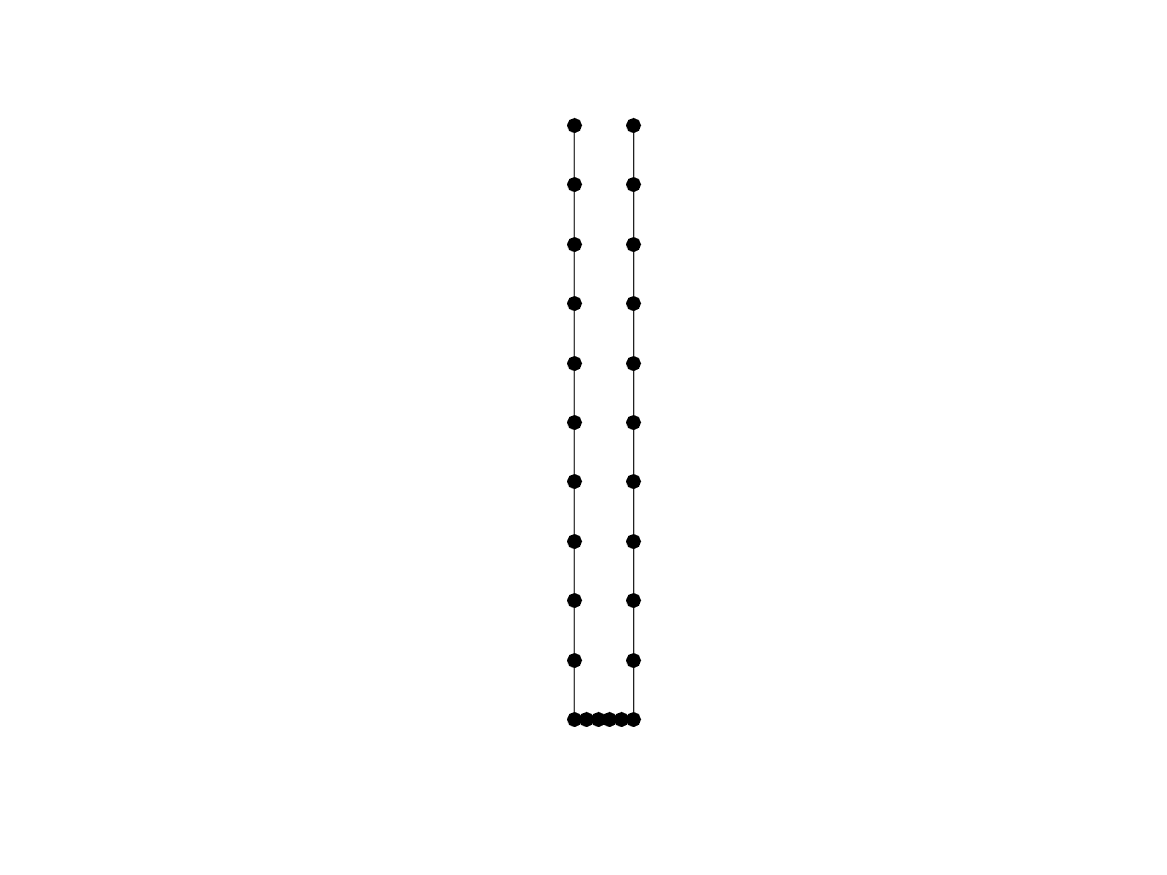
\includegraphics[width=\linewidth]{/Users/ole/Tex/MEK4420/oblig2images/boxes_4.png}
        \captionof{figure}{L/D = 0.1}
    \end{minipage}
\end{frame}

\begin{frame}
Vi ønsker å løse integrallikningen:
\begin{equation}\label{eq:144}
    -\pi \phi_2  + \int_{S_B} \phi_2 \frac{\partial G}{\partial n}  dS = \int_{S_B} G n_2 dS
\end{equation}
Men før vi gjør det vil vi sjekke at likningen fungerer. Så vi løser høyre- og venstresiden av en integrallikning der vi kjenner alle variablene. Vi ønsker å se om den reelle delen til høyresiden tilsvarer den reelle delen til venstresiden, og tilsvarende for de imaginære delene. 
\end{frame}

%her er det mulig å lime inn mere tekst og likninger.

%\subsection{Vi tester den numeriske løseren med KD=0.9}
\begin{frame}
\begin{minipage}[t]{0.45\linewidth}
    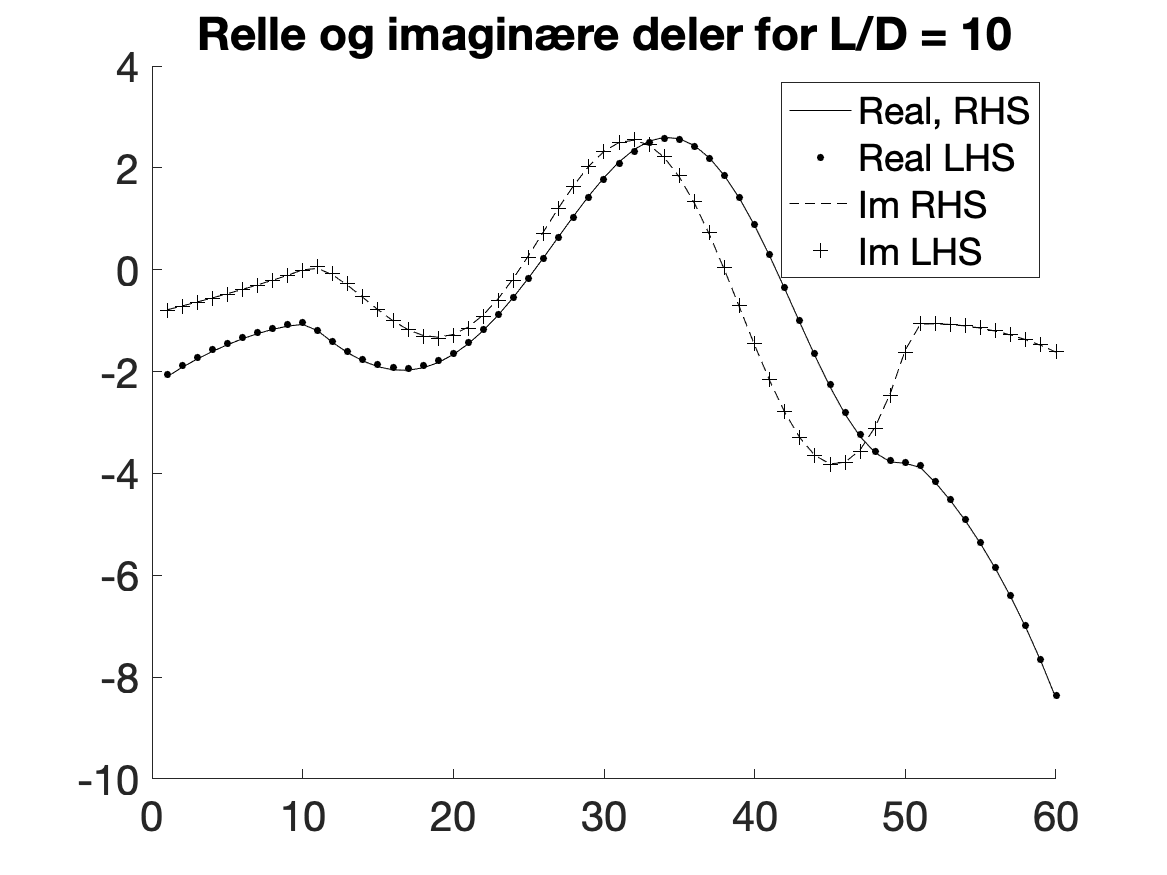
\includegraphics[width=\linewidth]{/Users/ole/Tex/MEK4420/oblig2images/plot_1_LD_1_nu09.png}
    \captionof{figure}{L/D = 10}
\end{minipage}
\hspace{0.05\linewidth}
\begin{minipage}[t]{0.45\linewidth}
    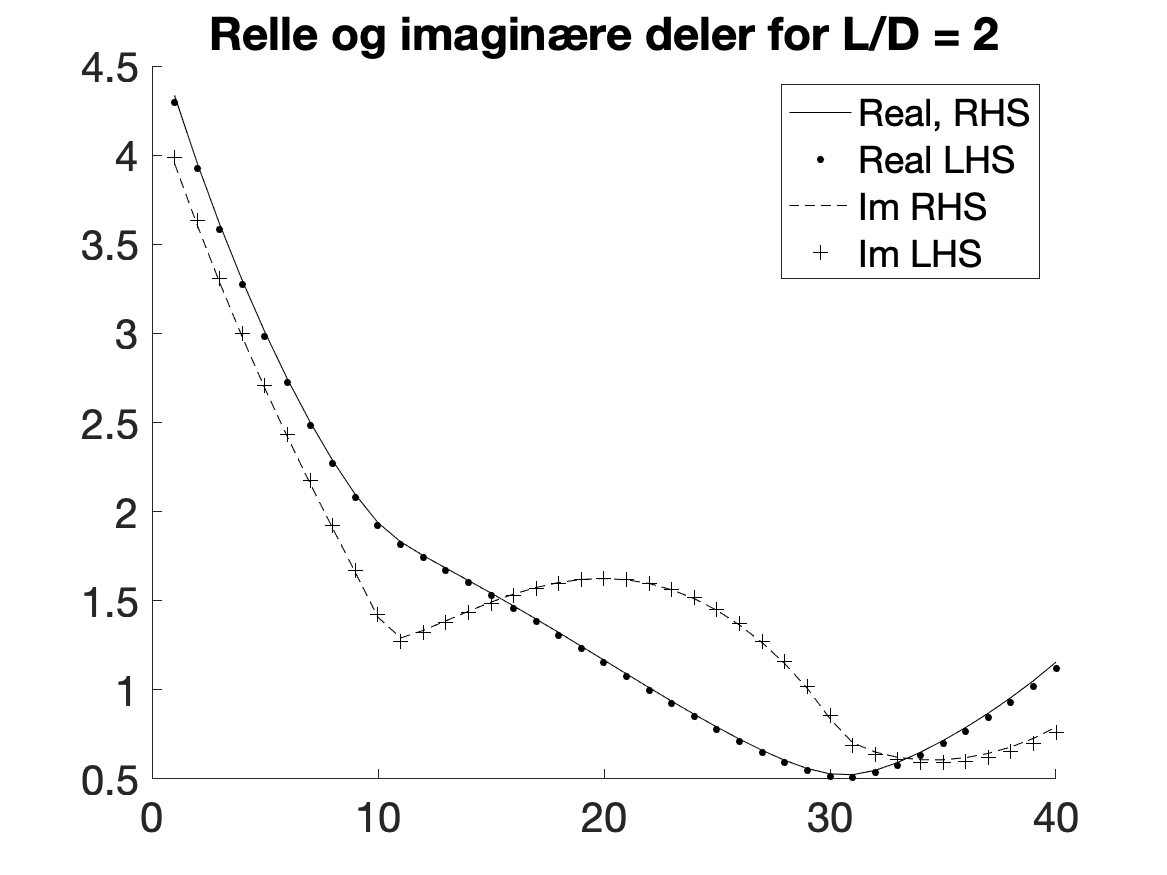
\includegraphics[width=\linewidth]{/Users/ole/Tex/MEK4420/oblig2images/plot_2_LD_2_nu09.png}
    \captionof{figure}{L/D = 2}
\end{minipage}
\begin{minipage}[t]{0.45\linewidth}
    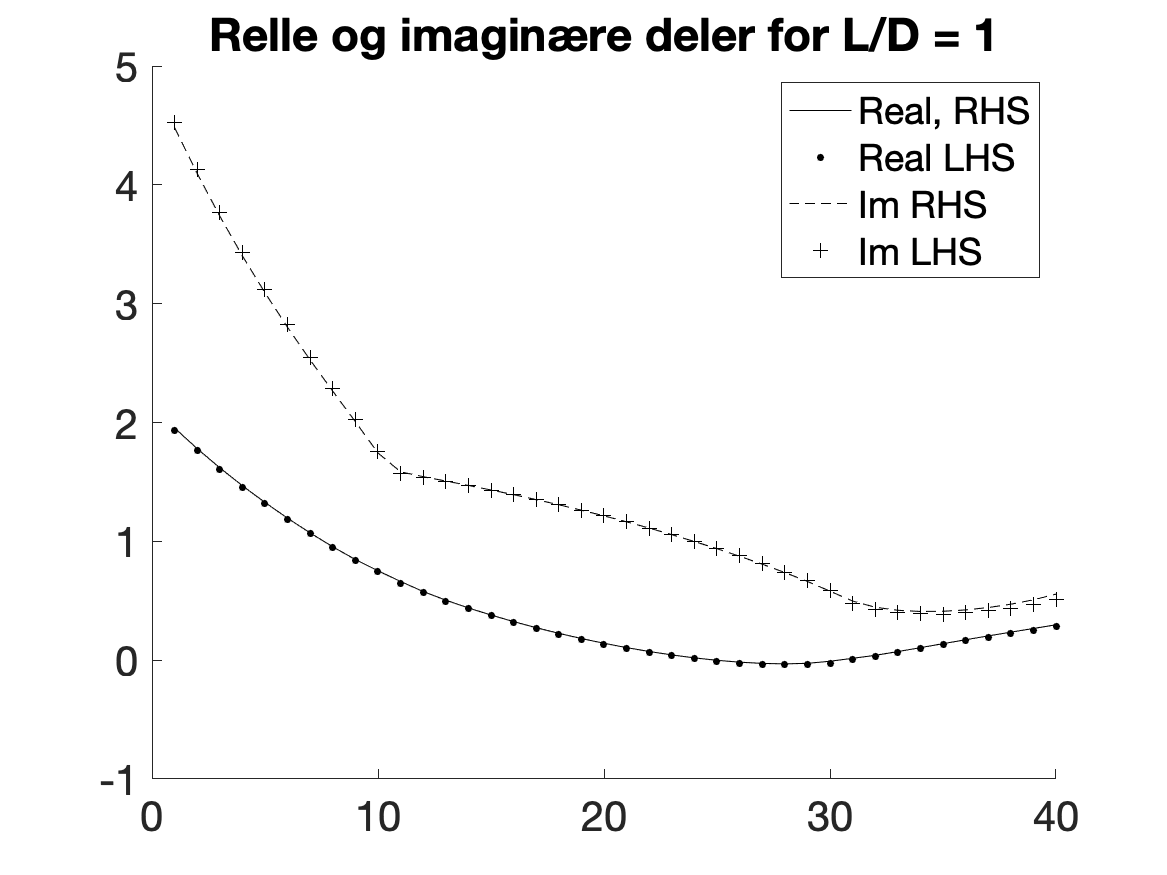
\includegraphics[width=\linewidth]{/Users/ole/Tex/MEK4420/oblig2images/plot_3_LD_3_nu09.png}
    \captionof{figure}{L/D = 1}
\end{minipage}
\hspace{0.05\linewidth}
\begin{minipage}[t]{0.45\linewidth}
    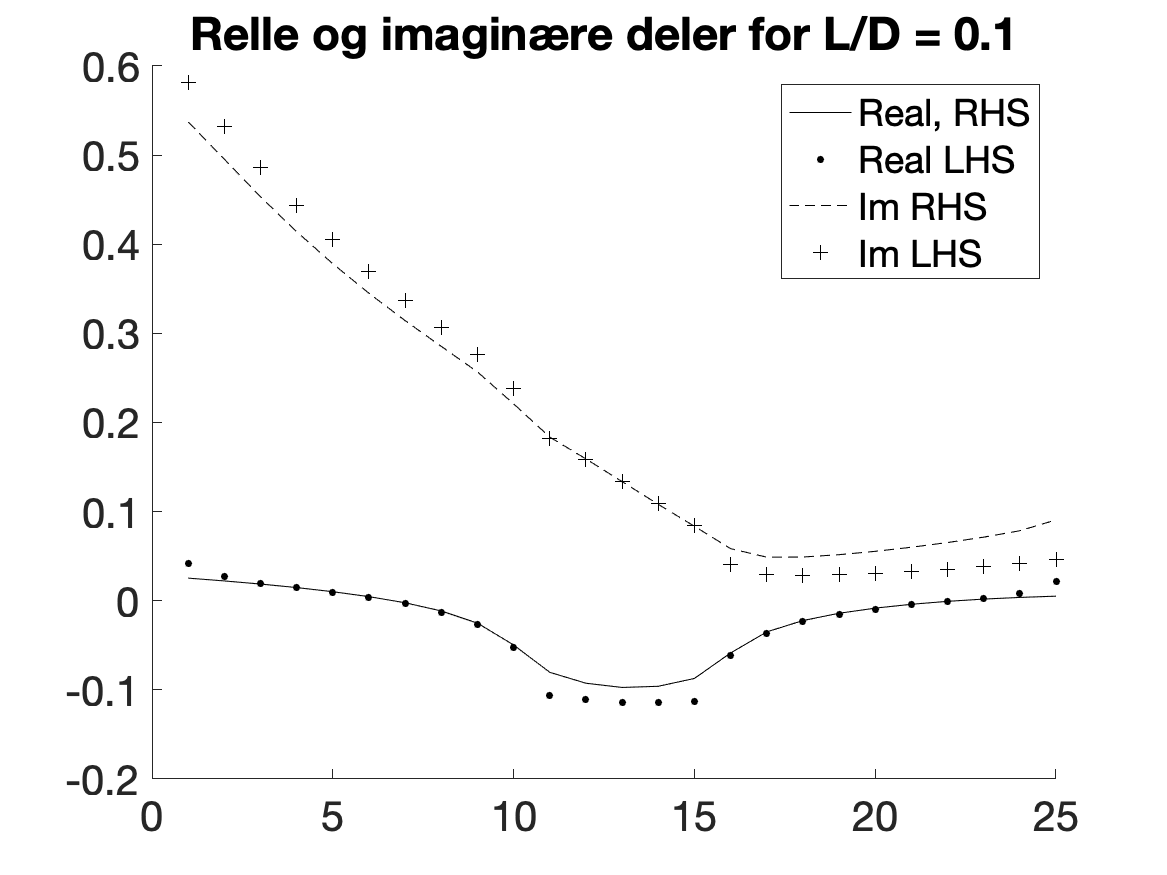
\includegraphics[width=\linewidth]{/Users/ole/Tex/MEK4420/oblig2images/plot_4_LD_4_nu09.png}
    \captionof{figure}{L/D = 0.1}
\end{minipage}
\end{frame}

%\subsection{Vi tester den numeriske løseren med KD=1.2}
\begin{frame}
\begin{minipage}[t]{0.45\linewidth}
    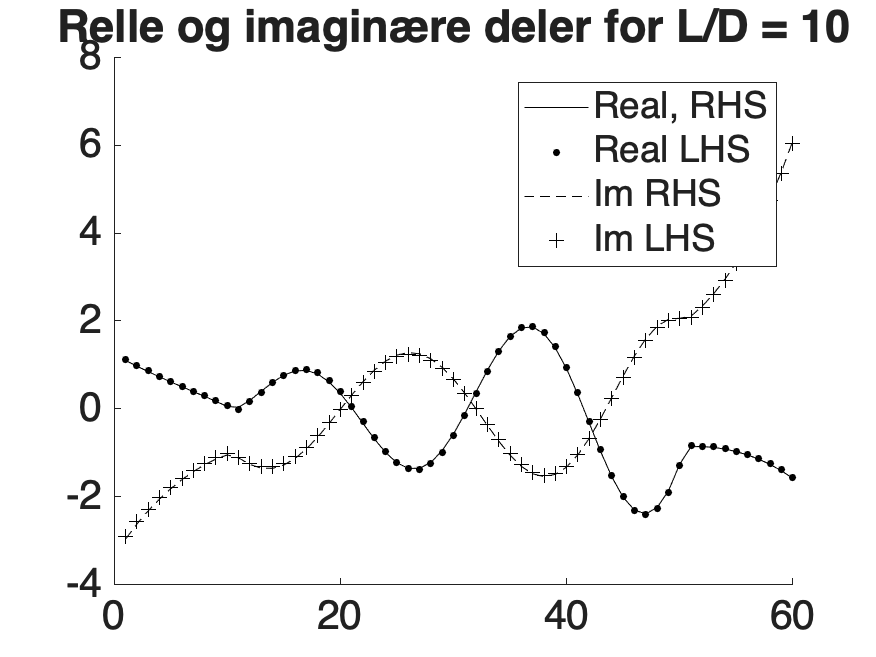
\includegraphics[width=\linewidth]{/Users/ole/Tex/MEK4420/oblig2images/plot_1_LD_1_nu12.png}
    \captionof{figure}{L/D = 10}
\end{minipage}
\hspace{0.05\linewidth}
\begin{minipage}[t]{0.45\linewidth}
    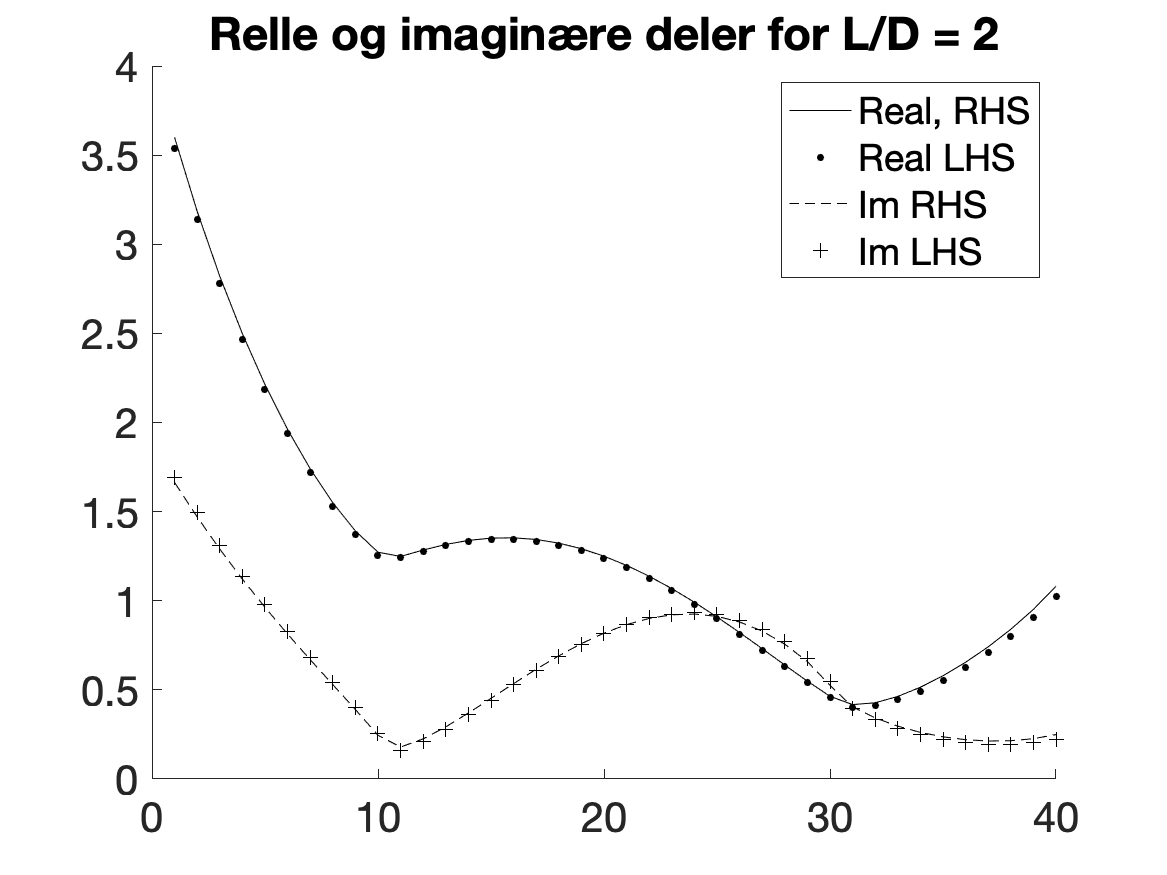
\includegraphics[width=\linewidth]{/Users/ole/Tex/MEK4420/oblig2images/plot_2_LD_2_nu12.png}
    \captionof{figure}{L/D = 2}
\end{minipage}
\begin{minipage}[t]{0.45\linewidth}
    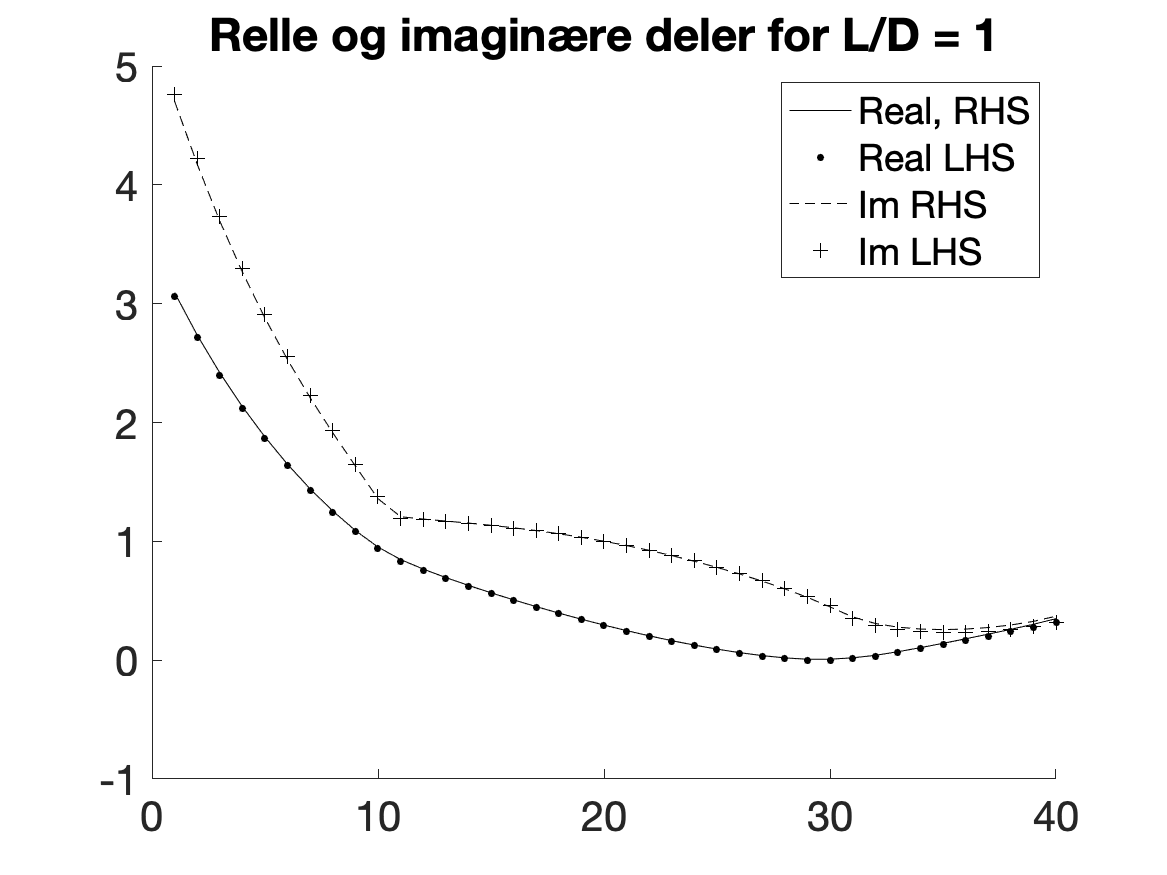
\includegraphics[width=\linewidth]{/Users/ole/Tex/MEK4420/oblig2images/plot_3_LD_3_nu12.png}
    \captionof{figure}{L/D = 1}
\end{minipage}
\hspace{0.05\linewidth}
\begin{minipage}[t]{0.45\linewidth}
    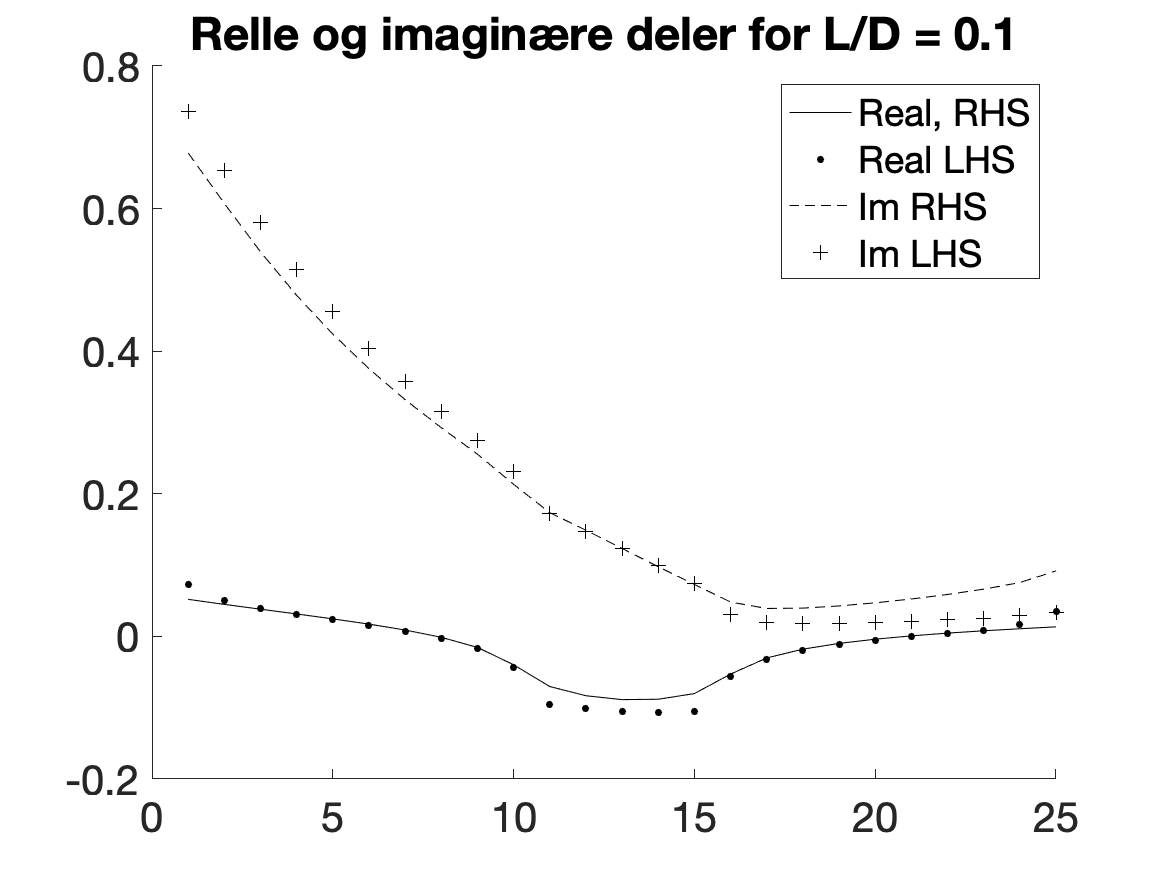
\includegraphics[width=\linewidth]{/Users/ole/Tex/MEK4420/oblig2images/plot_4_LD_4_nu12.png}
    \captionof{figure}{L/D = 0.1}
\end{minipage}
\end{frame}

% 7.5.3 Løsning av problemet i hiv
\begin{frame}
\frametitle{Løsning for potensialet i hiv}
%Så løser vi den originale likningen (\ref{eq:144}) numerisk for alle 4 geometriene. Og ser på plott av verdiene for potensialet $\phi_2$ på y-aksen. På x-aksen har vi de diskrete punktene. Plottet er symmetrisk fordi geometrien er symmetrisk.
\begin{minipage}[t]{0.45\linewidth}
    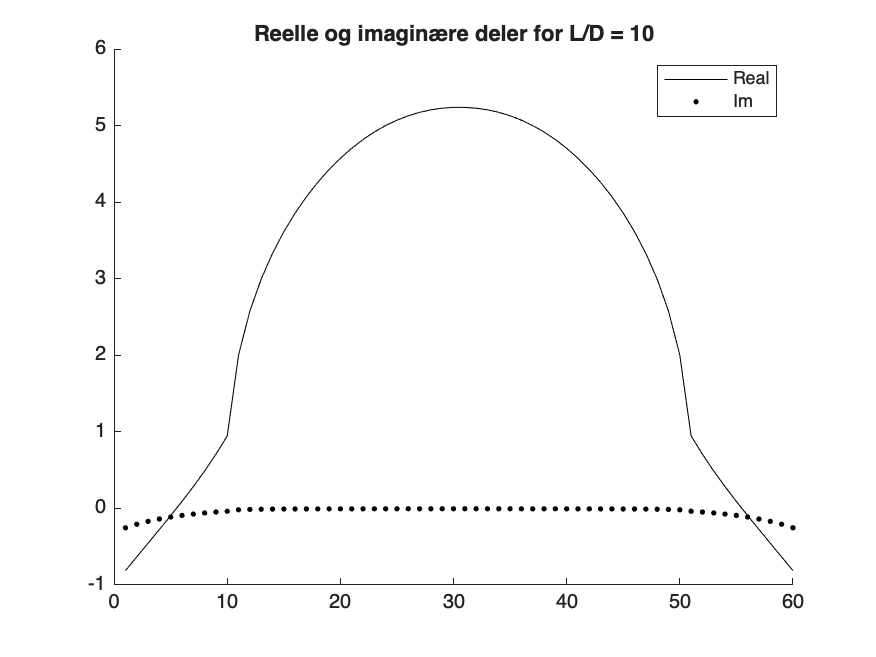
\includegraphics[width=\linewidth]{/Users/ole/Tex/MEK4420/oblig2images/plot_phi2_1.png}
    \captionof{figure}{L/D = 10}
\end{minipage}
\hspace{0.05\linewidth}
\begin{minipage}[t]{0.45\linewidth}
    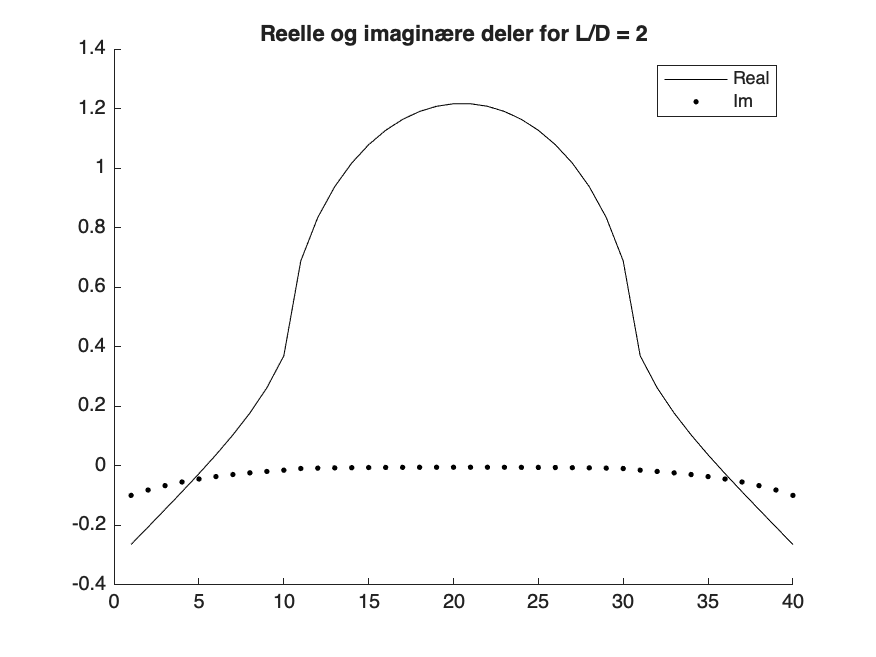
\includegraphics[width=\linewidth]{/Users/ole/Tex/MEK4420/oblig2images/plot_phi2_2.png}
    \captionof{figure}{L/D = 2}
\end{minipage}
\begin{minipage}[t]{0.45\linewidth}
    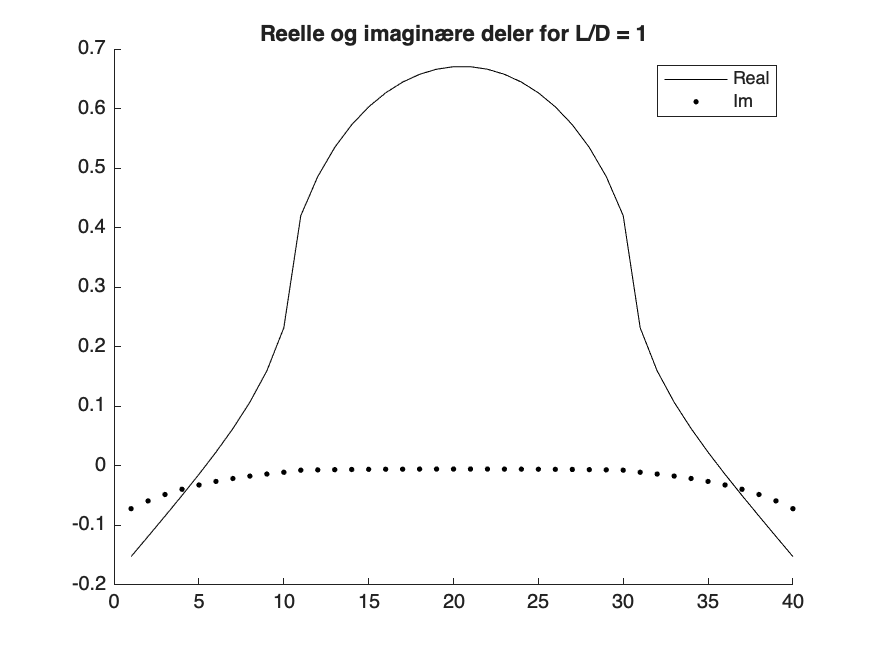
\includegraphics[width=\linewidth]{/Users/ole/Tex/MEK4420/oblig2images/plot_phi2_3.png}
    \captionof{figure}{L/D = 1}
\end{minipage}
\hspace{0.05\linewidth}
\begin{minipage}[t]{0.45\linewidth}
    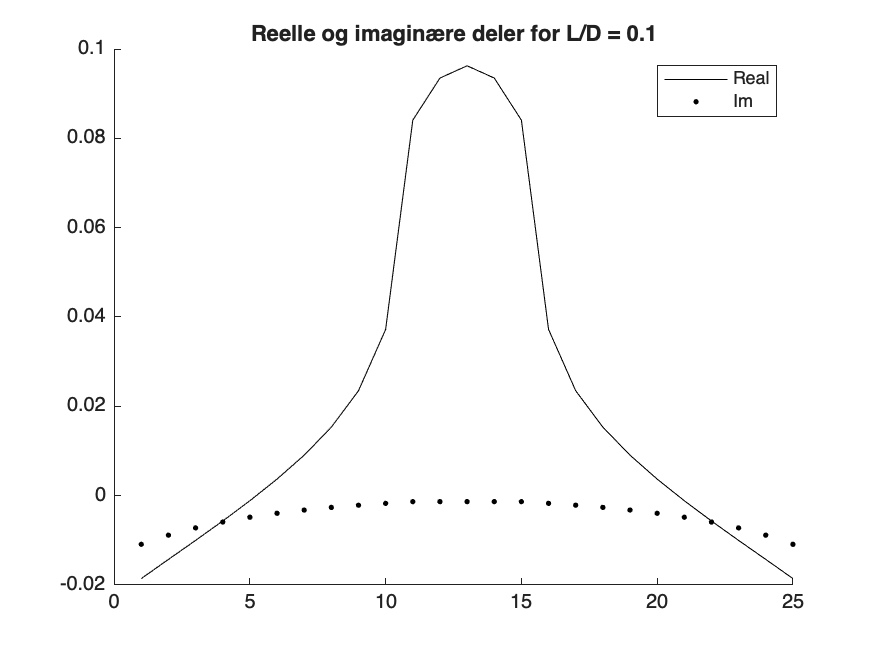
\includegraphics[width=\linewidth]{/Users/ole/Tex/MEK4420/oblig2images/plot_phi2_4.png}
    \captionof{figure}{L/D = 0.1}
\end{minipage}
\end{frame}

%  - 7.6 - Potensialet i fjernfeltet
\begin{comment}
\frametitle{.}
Langt borte har potensialet $\phi_2$  denne formen
\begin{align}
	\phi_2(\bar{x},\bar{y}) &\rightarrow A_2^{\pm \infty} e^{K\bar{y} + \mathrm{i} K\bar{x}}, \quad \bar{x} \rightarrow \pm \infty, 
\end{align}
fra likningen for fluidet så kan vi finne $A_2^{-\infty}$ og $A_2^{\infty}$
\begin{equation}
    2\pi \phi_2(\bar{x},\bar{y})  = \int_{S_B}  ( \phi_2  \frac{\partial G }{\partial n}-G n_2 )dS
\end{equation}
%avskrift fra side 32.
oppførselen til $\phi_j$ for $\bar{x} \rightarrow \pm \infty$,
\begin{align}
\phi_2 \rightarrow A_2^{\pm \infty} e^{K (\bar{y} \mp \mathrm{i}  \bar{x}) }, \quad \bar{x} \rightarrow \pm \infty.
\end{align}
%her har jeg byttet tre subscript fra j til 2.
Der de komplekse konstantene $A_2^{\pm \infty}$ finnes ved å ta integralet over svømmeflaten, som gir
\begin{align}
A_2^{\pm \infty} = \mathrm{i} \int_{S_B} \bigg(\phi_2 (n_1 \frac{\partial}{\partial x} + n_2  \frac{\partial}{\partial y}) - n_2 \bigg) e^{K(\bar{y} \pm \mathrm{i} \bar{x})} dS
\end{align}
\end{comment}

% 7.7 utgående bølgeamplitude  - COMMENT
\begin{comment}
Den utgående bølgeamplituden har komplekse amplituder,
\begin{align}
	amp_2^{\infty} = \xi_2 A_j^{ \infty} \frac{\omega^2}{g}, \quad \text{og} \quad amp_2^{-\infty} = \xi_2 A_j^{- \infty} \frac{\omega^2}{g}.
\end{align}
Gjennomsnittet av energifluksen til den utgående bølgen er gitt ved
\begin{align}
	\overline{\text{Energifluks}} = \bar{E}^{\infty}c_g + \bar{E}^{-\infty}c_g =  \frac{1}{2}\rho g {|amp_2|}^{\infty}c_g + \frac{1}{2}\rho g {|amp_2|}^{-\infty}c_g,
\end{align}
der $\bar{E}^{\pm \infty}$ er gjennomsnittlig energitetthet til utgående bølger og $c_g = \frac{\partial \omega}{\partial K}$ er gruppehastigheten. 
\end{comment}

% - - - % - - - % - - - % - - - % - - - % - - - %
\begin{frame}
\frametitle{Finne addert masse og dempning}
Vi bruker den numeriske løsningen til $\phi_2$ langs $S_B$ for å regne addert masse $a_{22}$ og dempning $b_{22}$. 
\begin{align}
F_{ij}(t) = - \rho \omega^2 \int_{S_B} \phi_i \hat{n}_j dS = - \omega^2 {\xi}_2 a_{22} + i \omega {\xi}b_{22}
\end{align}
Vi regner også ut $b_{22}$ fra energibalansen. 
\begin{align}
	\frac{1}{2} |\xi|^2 \omega^2 b_{22} =  {\bar{E}^{\infty} c_g + \bar{E}^{-\infty} c_g }
\end{align}
\begin{align}
	\frac{b_{22}}{\rho \omega} &=    \frac{1}{2}  ({| A_2^{\infty} |}^2 +  {| A_2^{-\infty}|}^2)
\end{align}
\end{frame}

\begin{frame}
%\subsection{Vi ser på addert masse og sammenlikner de to fremgangsmåtene for å finne $b_{22}$}
\begin{minipage}[t]{0.45\linewidth}
    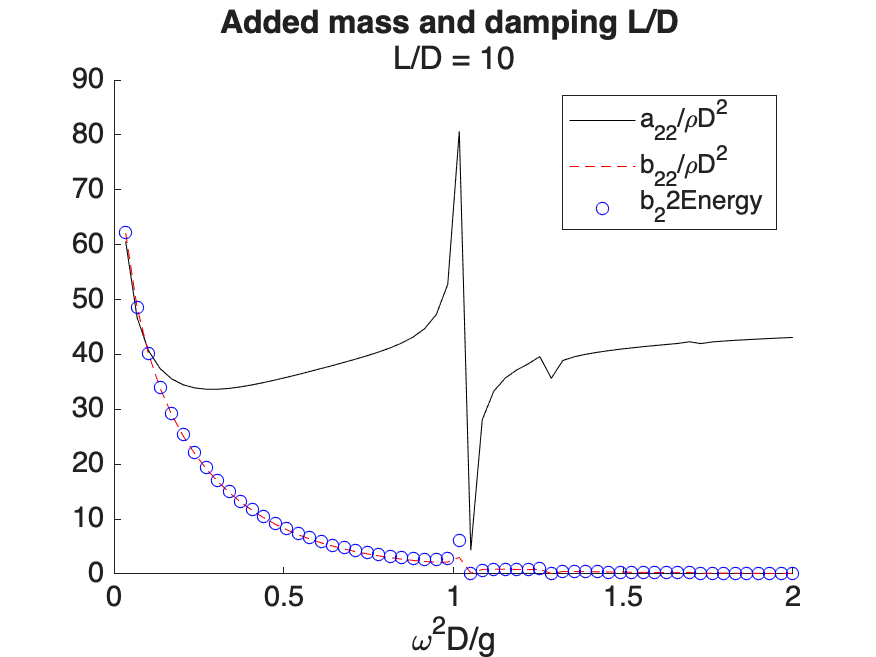
\includegraphics[width=\linewidth]{/Users/ole/Tex/MEK4420/oblig2images/plot_a22b22_1.png}
    \captionof{figure}{L/D = 10}\label{fig:a22_1}
\end{minipage}
\hspace{0.05\linewidth}
\begin{minipage}[t]{0.45\linewidth}
    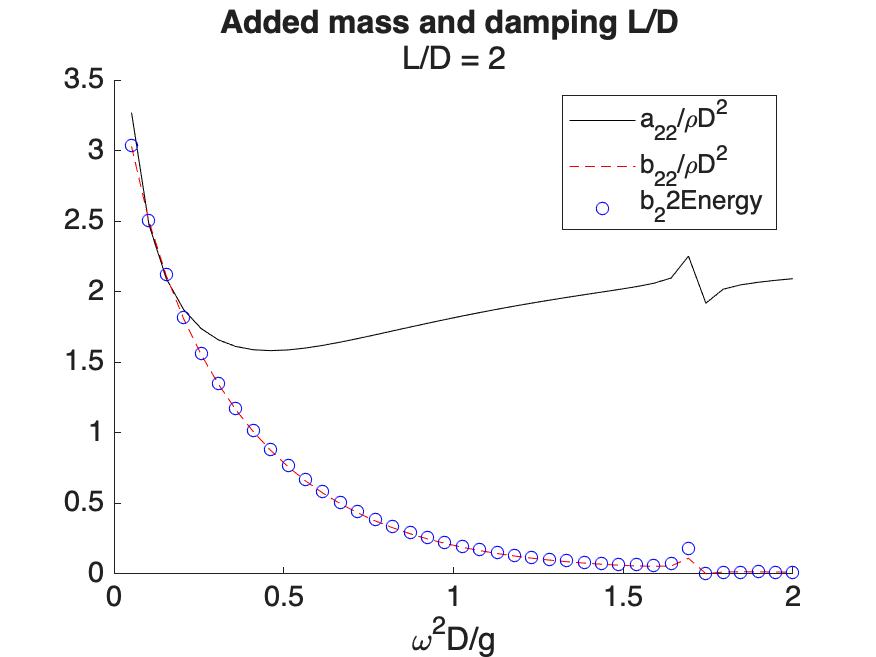
\includegraphics[width=\linewidth]{/Users/ole/Tex/MEK4420/oblig2images/plot_a22b22_2.png}
    \captionof{figure}{L/D = 2}\label{fig:a22_2}
\end{minipage}
\begin{minipage}[t]{0.45\linewidth}
    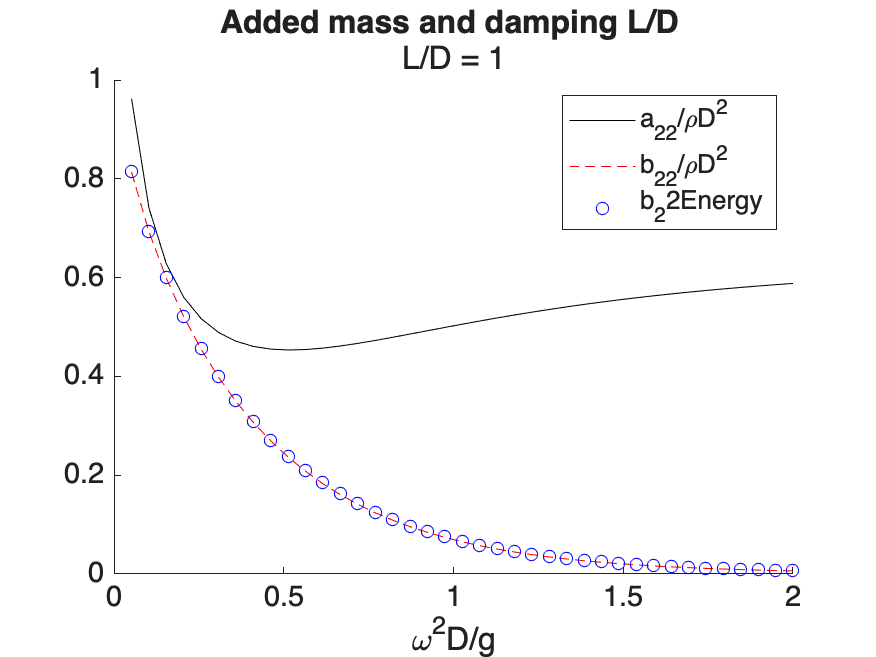
\includegraphics[width=\linewidth]{/Users/ole/Tex/MEK4420/oblig2images/plot_a22b22_3.png}
    \captionof{figure}{L/D = 1}\label{fig:a22_3}
\end{minipage}
\hspace{0.05\linewidth}
\begin{minipage}[t]{0.45\linewidth}
    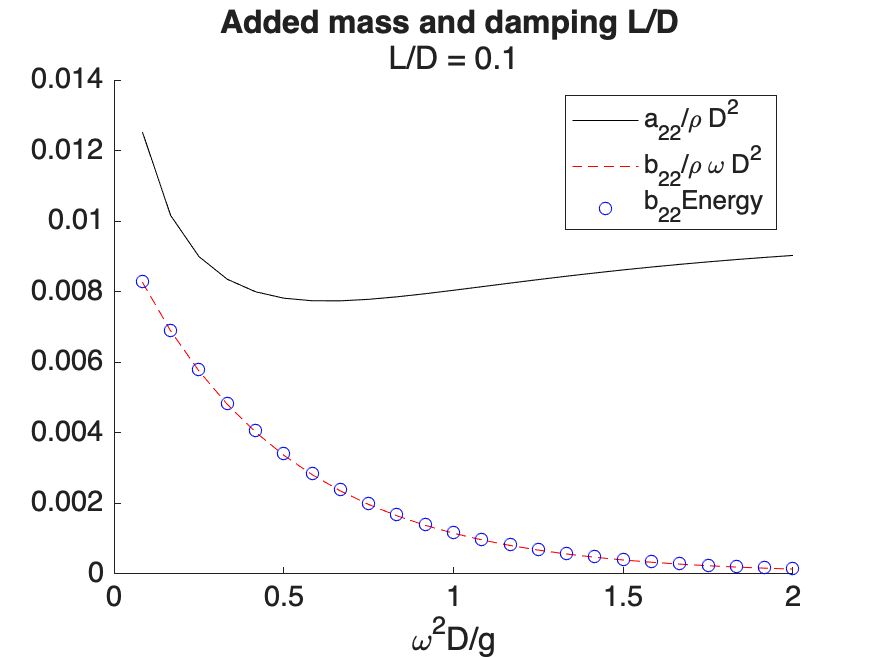
\includegraphics[width=\linewidth]{/Users/ole/Tex/MEK4420/oblig2images/plot_a22b22_4.png}
    \captionof{figure}{L/D = 0.1}\label{fig:a22_4}
\end{minipage} 
\end{frame}

% 7.9 Tilnærmet løsning 
\begin{frame}
\frametitle{Sparbøye - fritt flytende} 
Utgangspunkt fra Froude-Krylov approksimasjon for å estimere eksitasjonskraften. $D$ er dypgang og $L$ er lengden. % FK sin approx?
\begin{equation}
	X_2^{FK} = - \mathrm{i} \omega \rho \int_{S_B} \phi_0 n_2 dS = \rho g \int_{-L/2}^{L/2} e^{-KD- \mathrm{i}Kx} dx = \rho g L e^{-KD} \frac{\sin(KL/2)}{KL/2} 
\end{equation}
\begin{equation} 
	X_2^{FK} = \rho g L e^{-KD} , \quad \text{ fordi } \frac{\sin(KL/2)}{KL/2} \simeq 1,  \frac{KL}{2} \ll 1
\end{equation}
Vi har 
$c_{22} = \rho g L$. Fra Haskindrelasjonene finner vi dempningskoeffisienten: $\frac{b_{22}}{\rho \omega} = \frac{|X_2|^2 }{(\rho g)^2}$

Vi finner så responsen i hiv. 
\begin{align}
	(c_{22} - \omega^2(m_{22} + a_{22}) + \mathrm{i}\omega b_{22})\xi_2 &= AX_2 \\
	 \frac{\xi_{2}}{A} = \frac{ e^{-KD}}{ 1 - K D + \mathrm{i} K {L} e^{-2KD} }
\end{align}
\end{frame}


% 7.10 - Diffraksjonsproblemet
\subsection{Diffraksjonsproblemet}
\begin{frame}
 \frametitle{Diffraksjonsproblemet}
Geometrien holdes fast. Fluidets bevegelse er gitt ved 
\begin{equation}
\Phi_D(x,y,t) = Re\Big(A  \phi_D(x,y) e^{\mathrm{i} \omega t} \Big), 
\end{equation}
%der $A$ er amplituden og $\phi_0$ potensialet til innkommende bølger. Potensialet D finner vi fra $\phi_D(x,y) =  \phi_0(x,y) +  \phi_7(x,y)$. 
%$\phi_0(x,y) = \frac{\mathrm{i} g}{\omega}e^{Ky -\mathrm{i} K x}$. Og $K = \frac{\omega^2}{g}$. 
Spredningen $\phi_7$ er ukjent.

Integrallikningen vi bruker for å bestemme summen $\phi_D =  \phi_0 +  \phi_7$ til et punkt $(\bar{x},\bar{y})$ på $S_B$ er
\begin{equation}
    -\pi \phi_D(\bar{x},\bar{y})  + \int_{S_B}   \phi_D  \frac{\partial G }{\partial n}dS = -2\pi \phi_0
\end{equation}
\end{frame}

% 7.10 1og2. Eksitasjonskraft og Haskind.
\begin{frame}
\frametitle{Eksitasjonskraften}
Vi ønsker å finne eksitasjonskraften numerisk. %se side 301 Newman
\begin{equation}
	F_j(t)  =  \int_{S_B} - \rho \frac{\partial  \Phi_D }{\partial t }   n_j dS = Re(AX_j e^{\mathrm{i} \omega t})
\end{equation}
\begin{equation}
\frac{X_2}{\rho g}  =  -  \frac{\mathrm{i} \omega}{g}\int_{S_B}   \phi_D n_2dS
\end{equation}
\end{frame}

%SAMMENLIKNE EKSITASJONSKRAFT, HASKIND 1&2 OG FROUDE-KRYLOV
\begin{frame}
\frametitle{Haskindrelasjonene}
%Haskindrelasjonene 
%vi finner haskindrelasjonene ved å ta eksitasjonskraften, og bc dphi2dn = phi2. og så blir frie overflaten null, og  	
Første haskind-relasjon
\begin{equation}
\frac{X_2^{\text{Haskind v1}}}{i \omega \rho} = -\int_{S_B}  \big( \phi_0 \frac{\partial \phi_2}{\partial n} -\phi_2 \frac{\partial \phi_0}{\partial n}  \big) dS 
\end{equation}

Andre haskind-relasjon
\begin{equation}
\frac{X_2^{\text{Haskind v2}}}{i \omega \rho} = \int_{S_\infty}  \big( \phi_0 \frac{\partial \phi_2}{\partial n} -\phi_2 \frac{\partial \phi_0}{\partial n}  \big) dS =  \frac{\omega}{k} A_2^{-\infty}, 
\end{equation}
Fjernfeltet $\phi_2$ er gitt ved
\begin{align}
\phi_2 = A_2^{\pm \infty}e^{K ({y} \mp \mathrm{i}  {x}) },  \quad x \rightarrow\pm \infty
\end{align}
\end{frame}


\begin{frame}
%%%%- viser resultater under
%\subsection{Nå sammenlikner vi eksitasjonskraften ved direkte integrering, Haskind 1 og 2, og Froude-Krylov-tilnærmingen.}
\frametitle{Eksitasjonskraften}
\noindent
\begin{minipage}[t]{0.45\linewidth}
    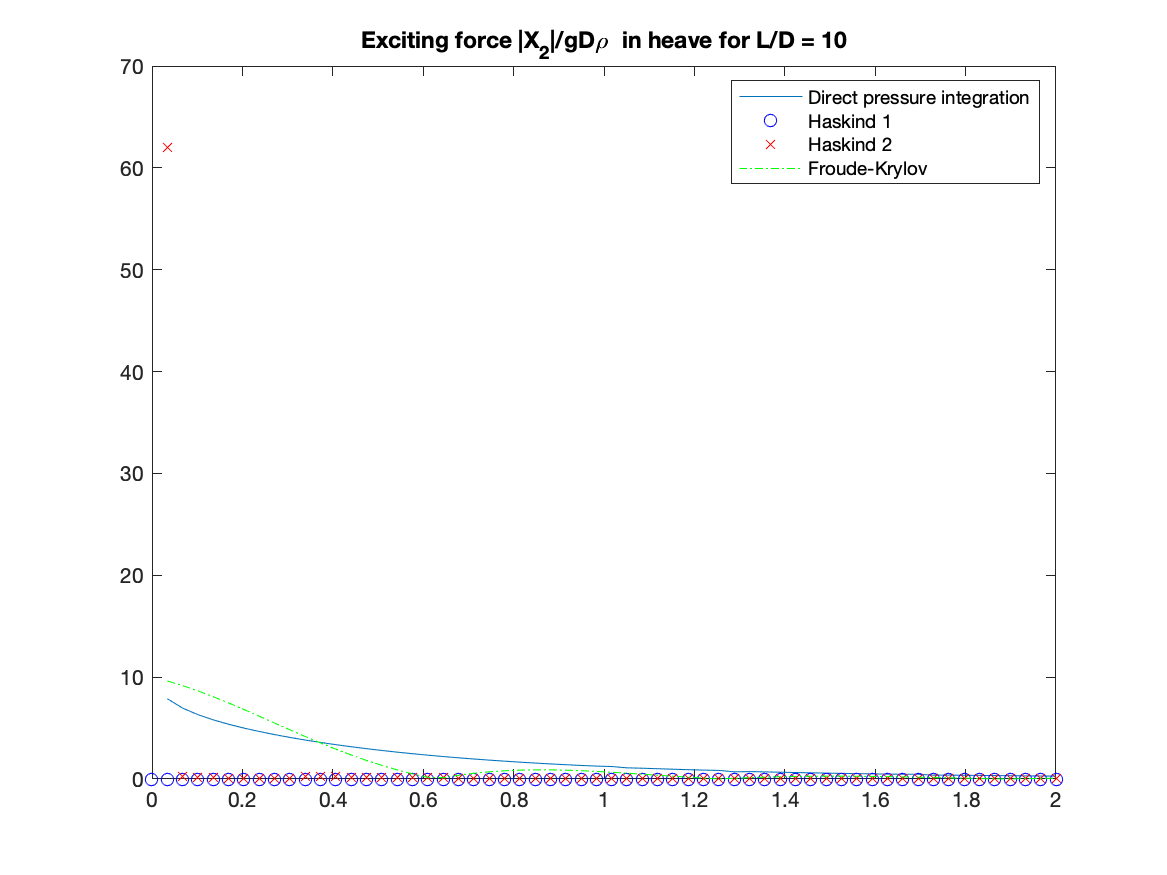
\includegraphics[width=\linewidth]{/Users/ole/Tex/MEK4420/oblig2images/aggregated_diffractionplot_1_LD_1.png}
    \captionof{figure}{L/D = 10}\label{fig:a22_1}
\end{minipage}
\hspace{0.05\linewidth}
\begin{minipage}[t]{0.45\linewidth}
    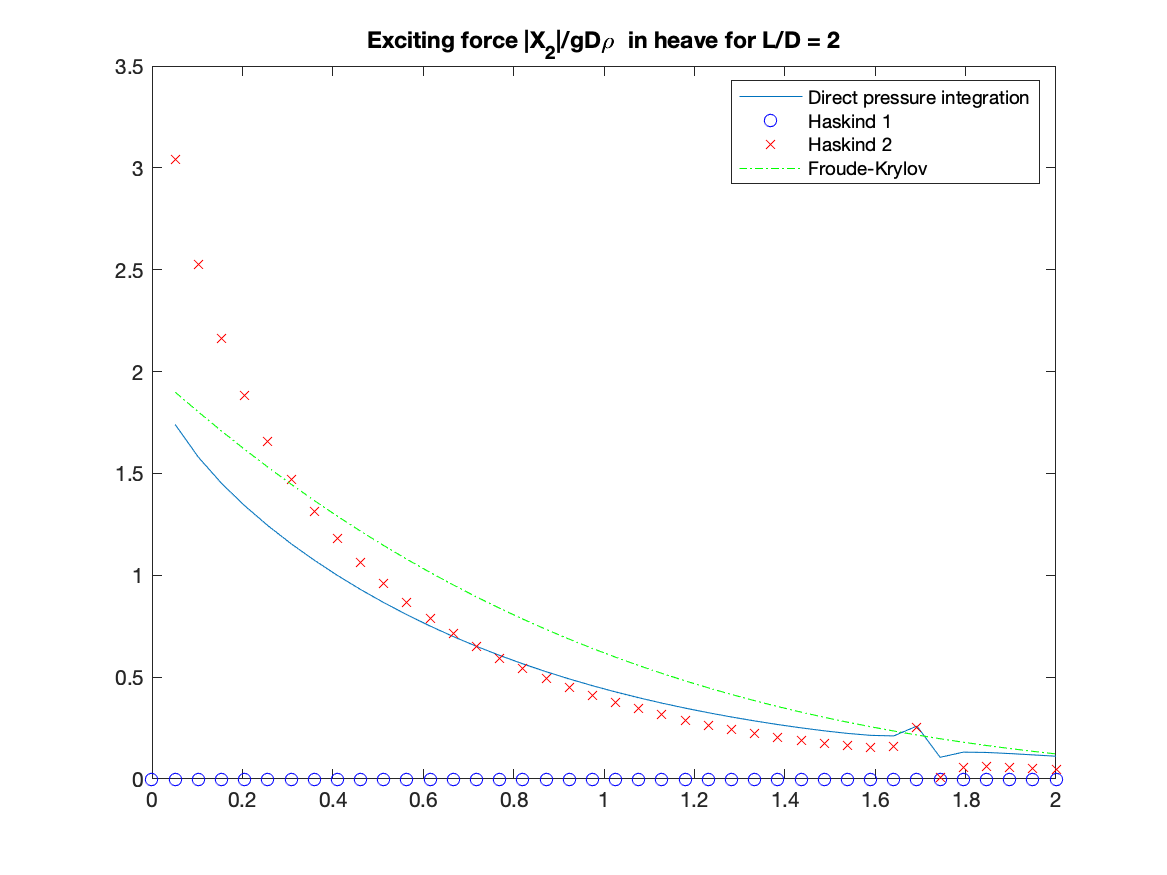
\includegraphics[width=\linewidth]{/Users/ole/Tex/MEK4420/oblig2images/aggregated_diffractionplot_2_LD_2.png}
    \captionof{figure}{L/D = 2}\label{fig:a22_2}
\end{minipage}
\vspace{-0.2cm} % removes vertical space between rows
\noindent
\begin{minipage}[t]{0.45\linewidth}
    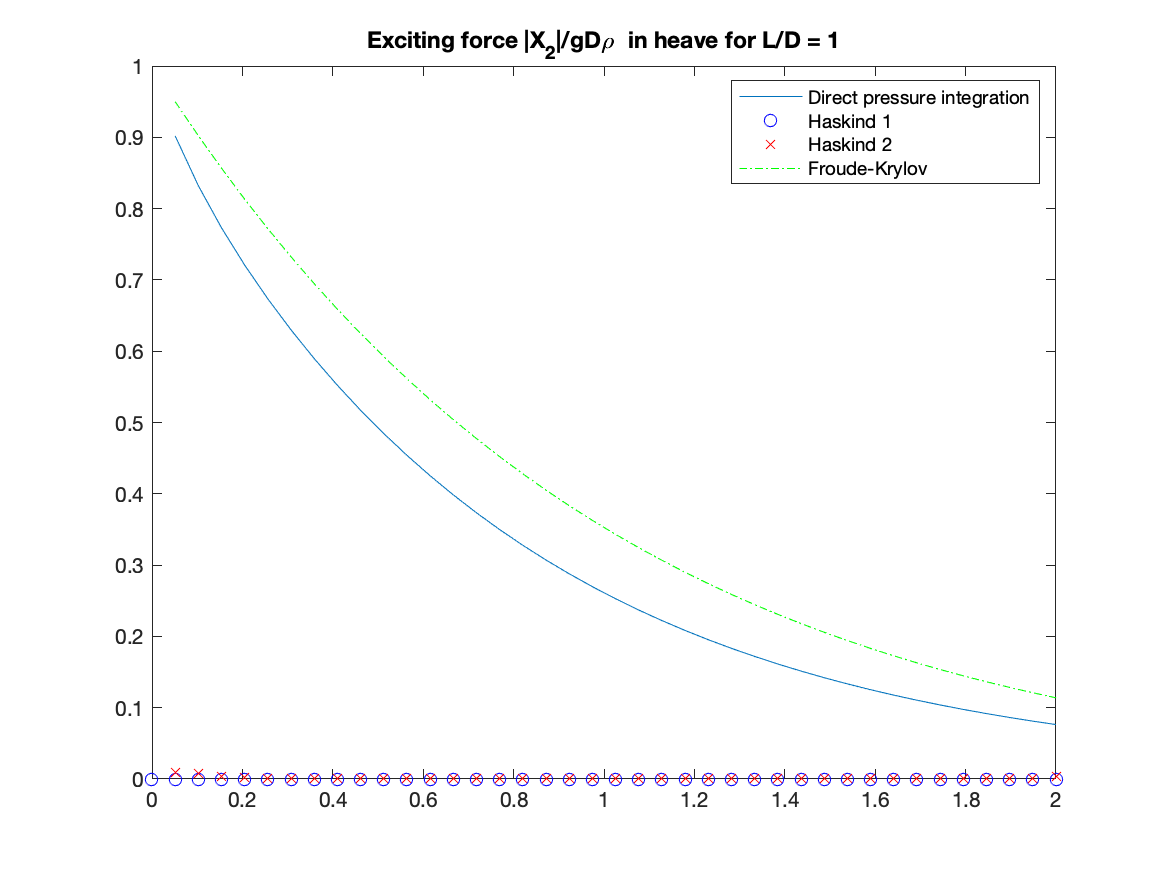
\includegraphics[width=\linewidth]{/Users/ole/Tex/MEK4420/oblig2images/aggregated_diffractionplot_3_LD_3.png}
    \captionof{figure}{L/D = 1}\label{fig:a22_3}
\end{minipage}
\hspace{0.05\linewidth}
\begin{minipage}[t]{0.45\linewidth}
    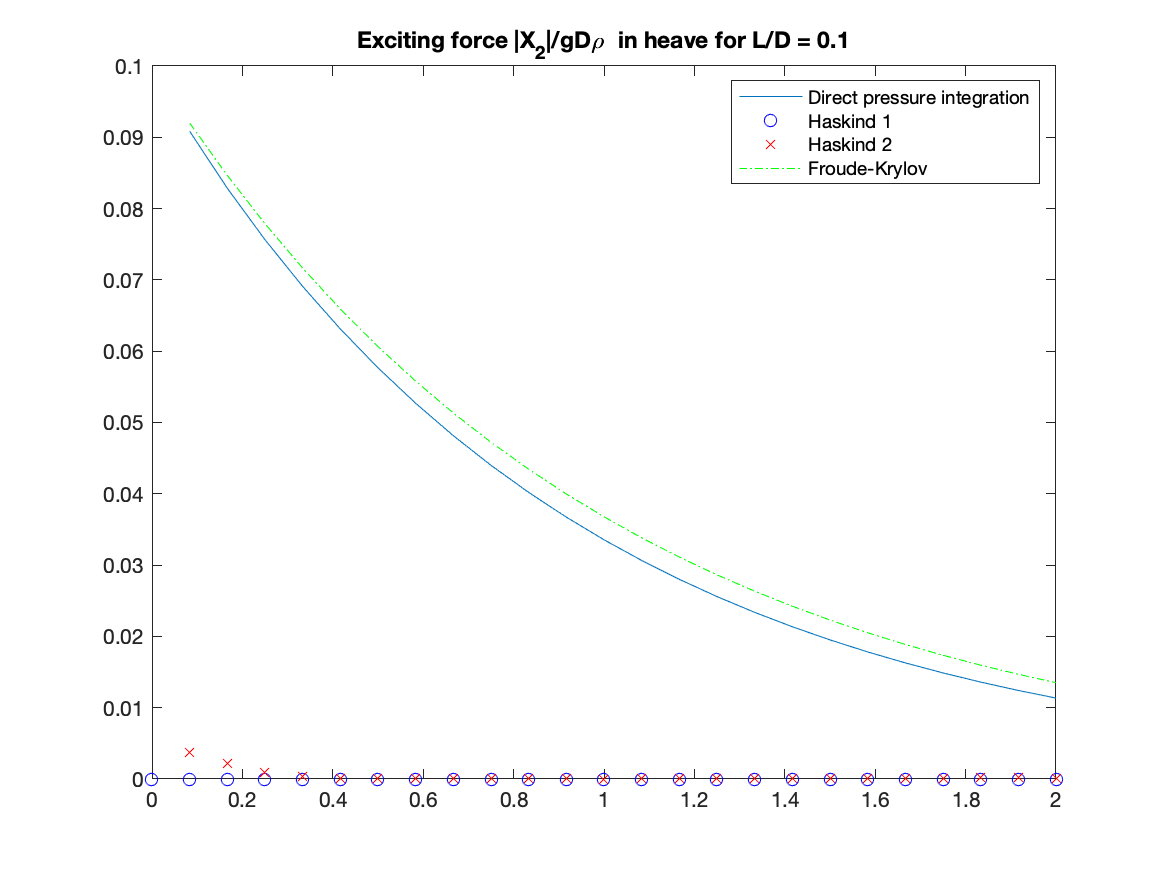
\includegraphics[width=\linewidth]{/Users/ole/Tex/MEK4420/oblig2images/aggregated_diffractionplot_4_LD_4.png}
    \captionof{figure}{L/D = 0.1}\label{fig:a22_4}
\end{minipage} 
\end{frame}

% 7.11 Respons i hiv -likning
\subsection{Respons i hiv}
\begin{frame}
\frametitle{Respons i hiv}
Likning for bevegelsen, kun i hiv, er gitt ved
\begin{equation}
( - \omega^2(m+a_{22}) + \mathrm{i}\omega b_{22}+ c_{22})\xi_2 = AX_2, 
\end{equation}
\begin{equation}
\frac{|\xi_2|}{A} = \frac{X_2}{c_{22} - \omega^2(m+a_{22}) + \mathrm{i}\omega b_{22}}, 
\end{equation}
der $c_{22} = \rho g S$. Svømmeflaten $S$ i vårt todimensjonale tilfelle er lengden på geometrien. $m$ er massen til geometrien, som for et fritt flytende legme er lik oppdriftskraften. Den adderte massen blir $a_{22} = \rho \forall = \rho LD$. $b_{22}$ er
\begin{equation}
b_{22} = \frac{K }{4\rho g V_g}|X_2|^2. 
\end{equation}
\end{frame}

% 7.11.1 Respons i hiv  - resonans. 
\begin{frame}
\frametitle{Resonansfrekvens}
Resonansfrekvensen $\omega_n$ oppstår der de hydrostatiske kreftene balanserer treghetskreftene, $c_{22}-\omega^2(m+a_{22}) = 0$. Resonansfrekvensen for en fritt flytende todimensjonal rektangulær seksjon med bredde L og dypgang D=1 blir, 
\begin{equation}
\omega^2_n = \frac{g}{D}  \frac{1}{1 + \frac{a_{22}}{\rho DL}}, 
\end{equation}
%For våre 4 geometrier finner vi addert masse fra figur \ref{fig:a22_1}, \ref{fig:a22_2}, \ref{fig:a22_3} og \ref{fig:a22_4}. 
\vspace{-0.9cm} 
\begin{table}%[htp]
\centering
\renewcommand{\arraystretch}{1.3} % Slightly increases row height
\caption{Resonansfrekvens}
\label{default}
\begin{tabular}{|p{1cm}|p{1cm}|p{1cm}|p{1cm}|p{1cm}|}
\hline
L/D & 10 & 2 & 1 & 0.1 \\ \hline
$a_{22}$ & 40 & 1.8 & 0.5 & 0.009 \\ \hline
$\frac{w_n^2}{g}$ & 0.2 & 0.53 & 0.67 & 0.92 \\ \hline
\end{tabular}
\end{table}
\end{frame}

% 7.11.2-3-4 Response as a function of frequency
\begin{frame}
%section{7.11.3}%section{7.11.4}%7.11.2-3-4 gir ett plott.
%Vi plotter responsen $\frac{|\xi|}{A}$ på tre måter. Først som en funksjon av frekvensen. Så, funnet ved Froude-Krylov-approksimasjonen $X_2^{FK}$, der $b_{22}$ finnes ved Haskind-relasjonene, og der effekten av addert masse $a_{22}$ er ignorert. Og til slutt, approksimasjonen, men justert for addert masse. Vi ser at verdiene for resonansfrekvensen tilsvarer toppene på kurvene våre.
\noindent
\begin{minipage}[t]{0.45\linewidth}
    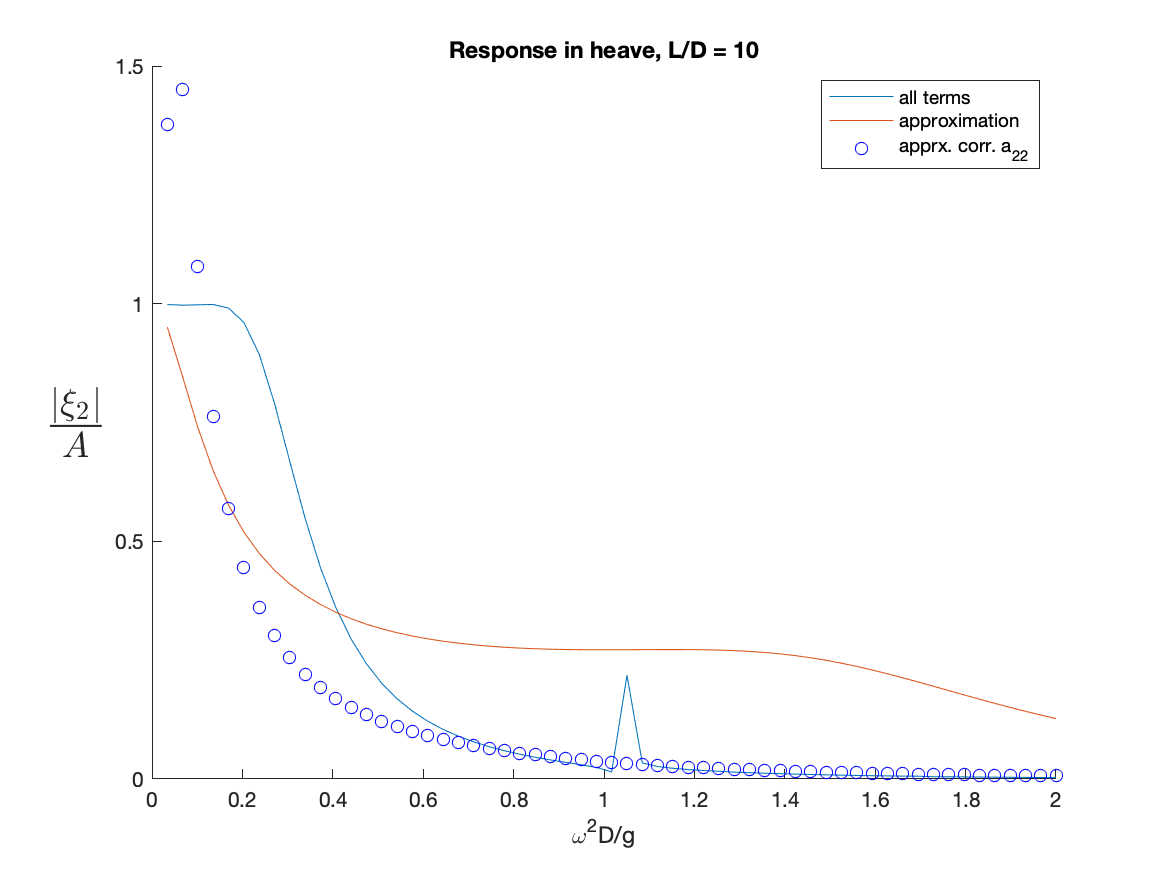
\includegraphics[width=\linewidth]{/Users/ole/Tex/MEK4420/oblig2images/rao_plot1_LD_1.png}
    \captionof{figure}{L/D = 10}
\end{minipage}
\hspace{0.05\linewidth}
\begin{minipage}[t]{0.45\linewidth}
    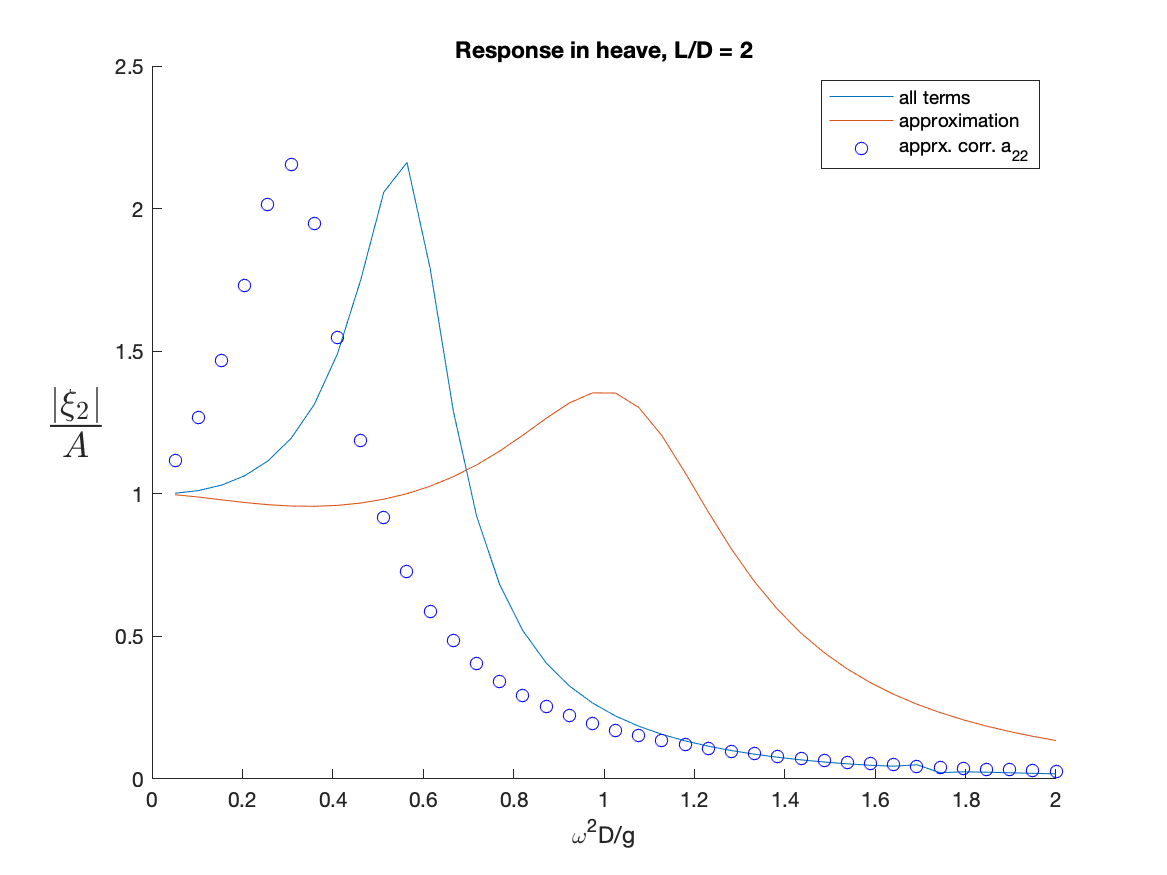
\includegraphics[width=\linewidth]{/Users/ole/Tex/MEK4420/oblig2images/rao_plot2_LD_2.png}
    \captionof{figure}{L/D = 2}
\end{minipage}
\noindent
\begin{minipage}[t]{0.45\linewidth}
    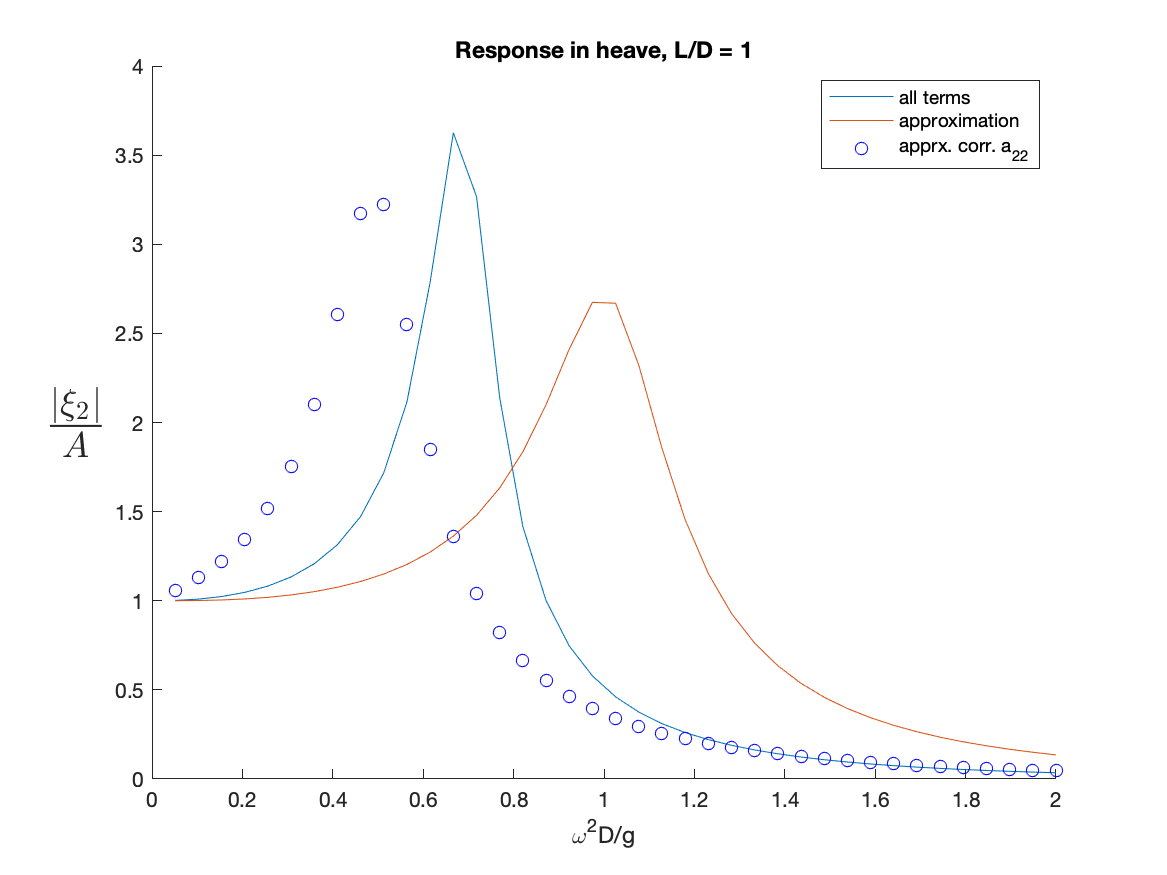
\includegraphics[width=\linewidth]{/Users/ole/Tex/MEK4420/oblig2images/rao_plot3_LD_3.png}
    \captionof{figure}{L/D = 1}
\end{minipage}
\hspace{0.05\linewidth}
\begin{minipage}[t]{0.45\linewidth}
    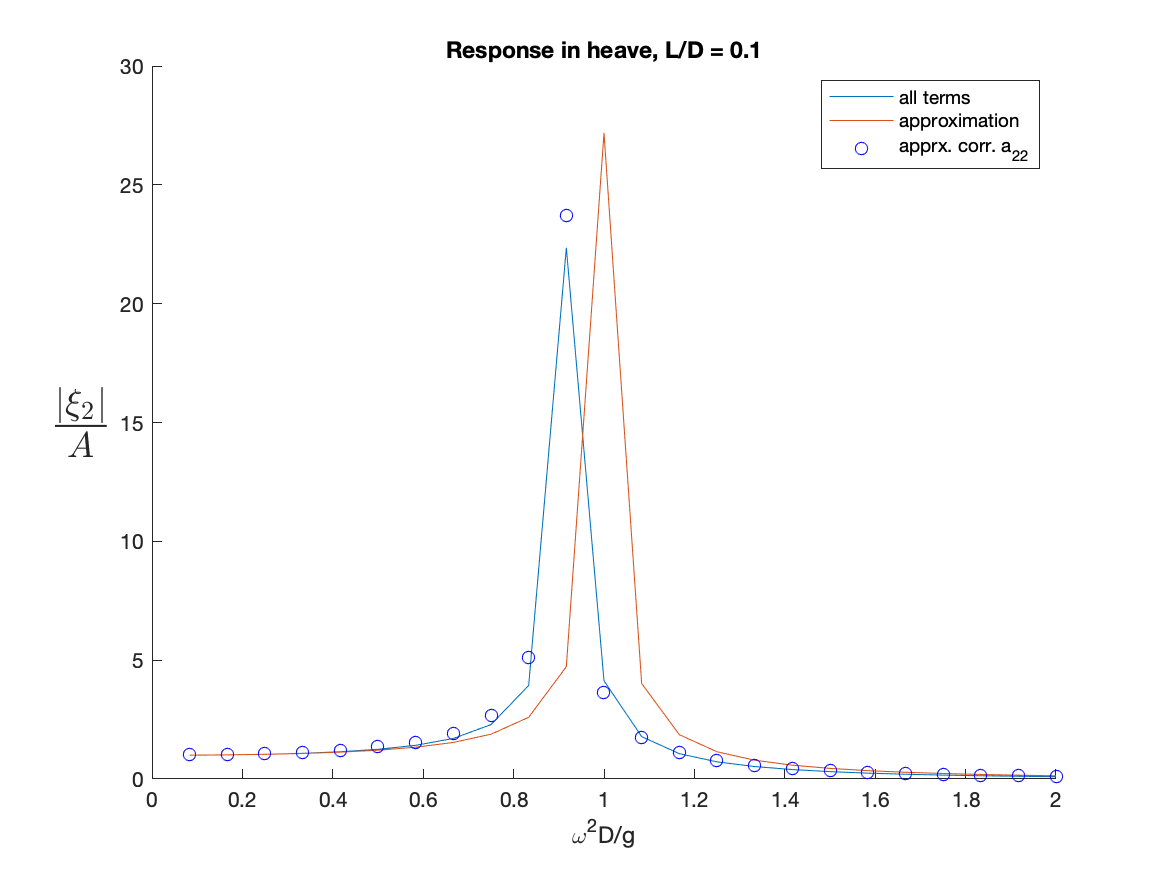
\includegraphics[width=\linewidth]{/Users/ole/Tex/MEK4420/oblig2images/rao_plot4_LD_4.png}
    \captionof{figure}{L/D = 0.1}
\end{minipage}
\end{frame}

% 
\begin{frame}
\centering
Takk for meg
\end{frame}

\end{document}
